\documentclass[12pt,a4paper]{report}
\usepackage[italian]{babel}

\usepackage[utf8]{inputenc}
\usepackage[T1]{fontenc}

\usepackage[parfill]{parskip}

\usepackage{booktabs}
\usepackage{textcomp}
\usepackage{graphics}
\usepackage{float}
\usepackage{color}
\usepackage{amsmath}
\usepackage{amssymb}
\usepackage{amsfonts}
\usepackage{hyperref}
\usepackage{cite}
\usepackage{calc}
\usepackage{enumitem}
%\usepackage{caption}
\usepackage{subcaption}
%\usepackage{pdfpages}
\usepackage{footnote}
\usepackage[bottom]{footmisc}
\usepackage{multirow}
\usepackage{threeparttable}
\usepackage{algorithm}
\usepackage[noend]{algpseudocode}
\usepackage{array}
\usepackage{rotating}
\usepackage{setspace}
\usepackage{wrapfig}
\graphicspath{{./images/}}

\captionsetup{compatibility=false}

\algnewcommand{\LineComment}[1]{\State{\(\triangleright\) #1}}
\algrenewcommand\Return{\State{\algorithmicreturn{} }}
\MakeRobust{\Call}


\begin{document}


\title{Titolo}
\author{Manuel Rota}

\begin{titlepage}
	\begin{onehalfspace}
	\begin{wrapfigure}[4]{l}[22mm]{0.25\textwidth}
		\vspace*{-7mm}
		\centering
		
\includegraphics[width=0.25\textwidth]{bicocca.png}
	\end{wrapfigure}
	\par
	Università degli Studi di Milano Bicocca \\
	\textbf{Scuola di Scienze \\
			Dipartimento di Informatica, Sistemistica e Comunicazione \\
			Corso di laurea in Informatica}
\end{onehalfspace}

\vfill
\par

\begin{doublespace}
\begin{center}
	{\Huge \textbf{Rilevamento di elementi testuali in immagini digitali}}
\end{center}
\end{doublespace}

\vfill
\par

\begin{onehalfspace}
\begin{flushleft}
	{\large \textbf{Relatore:} \textit{Prof.\ Raimondo Schettini} \\
	\textbf{Co-relatore:} \textit{Dott.\ Marco Buzzelli}}
\end{flushleft}

\vspace{8mm}
\par

\begin{flushright}
	{\large \textbf{Relazione della prova finale di:} \\
			\textit{Manuel Rota \\ Matricola 793785}}
\end{flushright}
\end{onehalfspace}

\vfill
\par

\begin{center}
	{\large \textbf{Anno Accademico 2016--2017}}
\end{center}


\end{titlepage}

\begin{abstract}
	Il rilevamento del testo in scene reali è un problema specifico della Computer Vision che negli anni è stato sempre oggetto di studi data la sua grande importanza, seppur mai completamente risolto al di fuori di applicazioni specifiche in condizioni controllate.
	In questa tesi analizziamo i diversi dataset a nostra disposizione per affrontare questo problema, introducendo brevemente anche le reti neurali con particolare attenzione alla loro utilizzo nell'ambito dell'object detection.
	Infine presentiamo vari dei nostri approcci sviluppati basati sulle \textit{Fully Convolutional Networks} confrontandoci con metodi concorrenti ed ottenendo risultati discreti ma al di sotto degli standard odierni, seppur promettenti e che in futuro potranno certamente migliorare applicando le novità recenti susseguitesi nello stato dell'arte.
\end{abstract}


\tableofcontents


\chapter{Introduzione}

Il rilevamento del testo è stato per molti anni una sfida impegnativa nel campo della Computer Vision, soprattutto qualora questo non si trovasse inquadrato come elemento principale in un'immagine o fosse ubicato in contesti caotici riscontrabili nella vita quotidiana.\par
Infatti, per molti decenni le uniche implementazioni di tali metodi furono sempre rilegate a compiti molto ristretti e in condizioni prevedibili, come per esempio la localizzazione, estrazione e riconoscimento di parole in documenti stampati o scritti a mano, raggiungendo così risultati sì considerevoli, ma solo all'interno della specifica applicazione.\par
Scopo di questa tesi, come quello della ricerca in questo campo negli ultimi anni, è dunque il rafforzamento del task di \textbf{text detection} applicato a immagini raffiguranti i più vari contesti di scene reali andando a studiare ed applicare alcuni dei più recenti strumenti a nostra disposizione.\par

\vspace{10pt}

\section{Competizioni}
Nel corso degli anni, al fine di incentivare la ricerca in questo campo, sono nate molte competizioni riguardanti l'argomento in studio nelle sue più varie sfaccettature.\par
L'\textbf{International Conference on Document Analysis and Recognition}~\cite{ICDAR} (ICDAR), è una conferenza internazionale la quale dal 1991 a cadenza biennale raggruppa varie di queste competizioni.\par
Molti di queste sono strutturate perlopiù nei seguenti task individuali:
\begin{itemize}
	\item Text Localization: \\
		Ottenimento di un'area approssimativa occupata dalle zone di testo
	\item Test Segmentation: \\
		Segmentazione dei singoli caratteri dallo sfondo
	\item Word Recognition: \\
		Raggruppamento dei caratteri in parole e loro trascrizione
\end{itemize}
\vspace{4pt}
La fase di interesse di questa tesi è quella di \textit{Text Localization}.

\section{Stato dell'Arte}
\label{sec:sota}
Negli anni molti metodi hanno tentato di approcciarsi a questo problema, adottando solitamente una fase di localizzazione dei singoli caratteri seguita da un loro raggruppamento in parole. Tra i più recenti possiamo citare:
\begin{itemize}
	\item
		\textbf{TextFlow}~\cite{tian2015text} \\
		Fast Cascade Boosting seguito da una rete di flusso dei costi minimi.
	\item
		\textbf{Canny Text Detector}~\cite{cho2016canny} \\
		 Regioni estremali stabili massimamente (MSER) con AdaBoost per l'eliminazione di falsi positivi.
\end{itemize}

Recentemente però, con la crescita in popolarità e delle prestazioni delle reti neurali, ed in particolare quelle convoluzionali nel campo dell'object detection, sono nati molti altri metodi anche fra di loro differenti, fra i quali possiamo citare:
\begin{itemize}
	\item \textbf{Multi-Oriented Text Detection}~\cite{zhang2016multi} \\
		Region proposal con Convolutional Neural Networks seguita da metodi ``tradizionali''
	\item \textbf{WordFence}~\cite{polzounov2017wordfence} \\
		Separazione delle zone proposte come testo con la predizione dei bordi delle parole
	\item \textbf{Deep Direct Regression}~\cite{he2017deep} \\
		Proposta di zone di interesse e regressione delle singole bounding box
\end{itemize}


\section{Struttura della tesi}
Questa tesi è strutturata nei seguenti capitoli principali:
\begin{enumerate}
\setcounter{enumi}{1}
	\item \textbf{Dataset e Competizioni} \\
		Questo capitolo descrive i vari dataset pubblici utilizzati, sia per una nostra fase di addestramento che per la valutazione dei nostri metodi, analizzando le tecniche di misurazione di performance utilizzate. 
	\item \textbf{Reti Neurali} \\
		Questo capitolo copre in breve la storia e teoria delle reti neurali dalla loro concezione fino ai giorni nostri, per arrivare al loro utilizzo odierno nel campo della Computer Vision per l'object detection.
	\item \textbf{Esperimenti} \\
		Questo capitolo illustra i nostri approcci incrementali al problema dela Text Localization con le tecniche di \textit{deep learning} illustrate nel capitolo precedente.
	\end{enumerate}


\chapter{Dataset e Competizioni}

Nonostante negli anni nel mondo della Computer Vision vi sia sempre stata una necessità di dataset pubblici per la comparazione di metodi concorrenti, i dati a disposizione su cui lavorare sono stati invece relativamente esigui poiché la gran parte dei problemi venivano solitamente risolti con un approccio di tipo analitico.\par
Da quando però nell'ultima decade è avvenuto un cambiamento nel modo di porsi a molte sfide grazie all'adozione delle reti neurali come strumento per l'apprendimento automatico, questa esigenza, aiutata anche dell'arrivo dei cosiddetti \textit{Big Data}, si è espansa in svariati settori dell'informatica.\par 
Il bisogno sempre più crescente di dati, nella nostra area di interesse di tipo visivo, però non è esente da problematiche: per l'apprendimento automatico sono infatti richiesti dati costituenti una \textit{groundtruth}, ovvero informazioni che rappresentino verosimilmente la soluzione del problema postosi, e perciò non generabili in gran quantità ed automaticamente da un elaboratore.\par
Dataset degni di nota nel campo della Computer Vision che si sono imposti come standard nell'ambito dell'\textit{object detection} sono il PASCAL Visual Object Classes~\cite{pascalvoc}, ImageNet~\cite{imagenet} ed il più recente MSCOCO~\cite{mscoco}.\par
Di seguito approfondiremo i vari dataset a nostra disposizione per il task della localizzazione del testo e i principali metodi di valutazione proposti nella letteratura e adottati da varie competizioni.

\section{Dataset}

\subsection{Focused Scene Text}
\label{subsec:focused}
Introdotto per la prima volta in occasione di ICDAR2013~\cite{ICDAR2013}, è composto da immagini acquisite in contesti reali dove l'oggetto principale è un'area di testo, solitamente orizzontale e formata da caratteri alfanumerici.\\
Nasce quindi avendo in mente i casi d'uso più comuni, quali la lettura del testo ed eventualmente una sua traduzione, portando dunque in secondo piano la fase di localizzazione, resa più immediata, a favore di un focus sulla precisa segmentazione e riconoscimento delle singole parole e/o lettere.\par
Caratteristiche:
\begin{itemize}
	\item
		229 immagini di training
	\item
		233 immagini di test
	\item
		groundtruth composta dalle coordinate delle bounding box ortogonali e trascrizione di ogni singola parola
\end{itemize}

\subsection{Incidental Scene Text}
\label{subsec:incidental}
Introdotto per la prima volta nell'omonima competizione in occasione della conferenza ICDAR2015~\cite{ICDAR2015}, è composto da immagini acquisite in contesti reali (attraverso fotocamere indossabili) dove le aree di testo non sono l'oggetto principale e possono dunque trovarsi a diverse distanze e posizioni.\\
Questa differenza con il dataset precedente lo rende più adatto come metro di valutazione per il task su cui ci concentreremo in questa tesi in quanto la fase di localizzazione viene resa meno triviale. Verrà usato anche per la comparazione con metodi concorrenti.\par
Caratteristiche:
\begin{itemize}
	\item
		$1000$ immagini di training
	\item
		$500$ immagini di test
	\item
		groundtruth composta dalle coordinate dei vertici delle bounding box orientate e trascrizione di ogni singola parola (quando leggibile)
\end{itemize}


\begin{figure}[H]
	\centering
	\begin{subfigure}[b]{0.4\textwidth}
		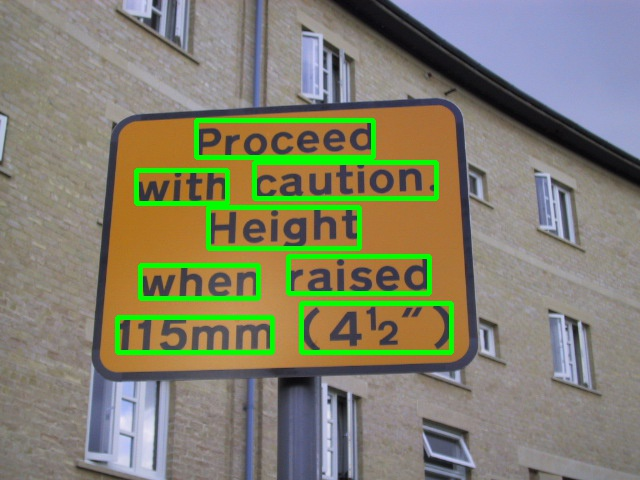
\includegraphics[width=\textwidth,trim={2cm 0 4cm 0},clip]{focused_example.jpg}
		\caption{Focused Text Scene}
	\end{subfigure}
	\hfill
	\begin{subfigure}[b]{0.55\textwidth}
		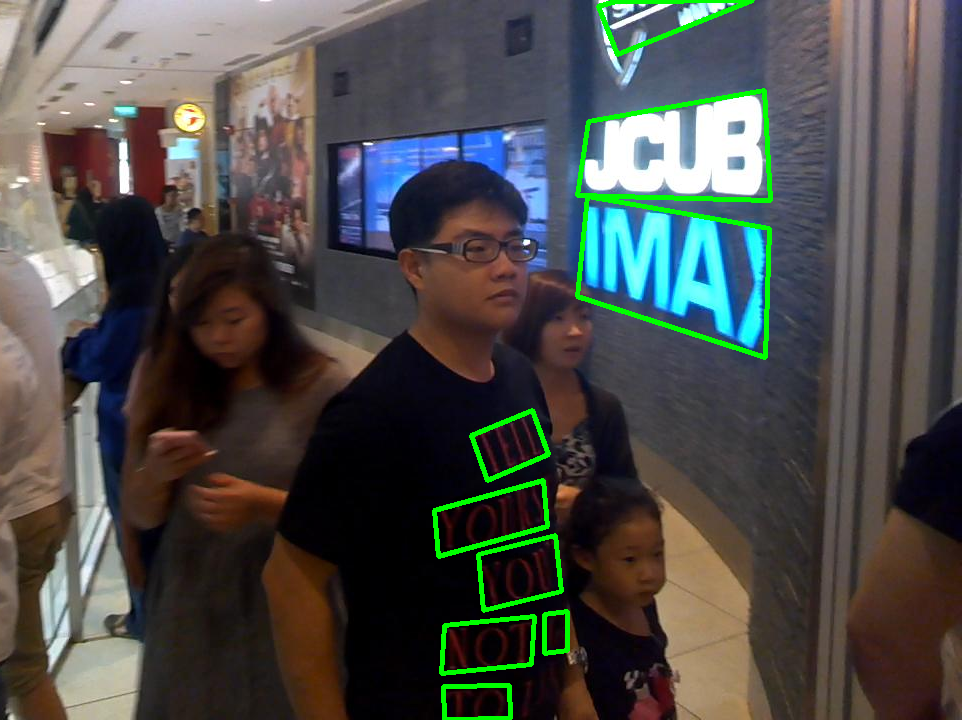
\includegraphics[width=\textwidth]{incidental_example.png}
		\caption{Incidental Text Scene.}
	\end{subfigure}
	\caption{Immagini di training con relative annotazioni.}
	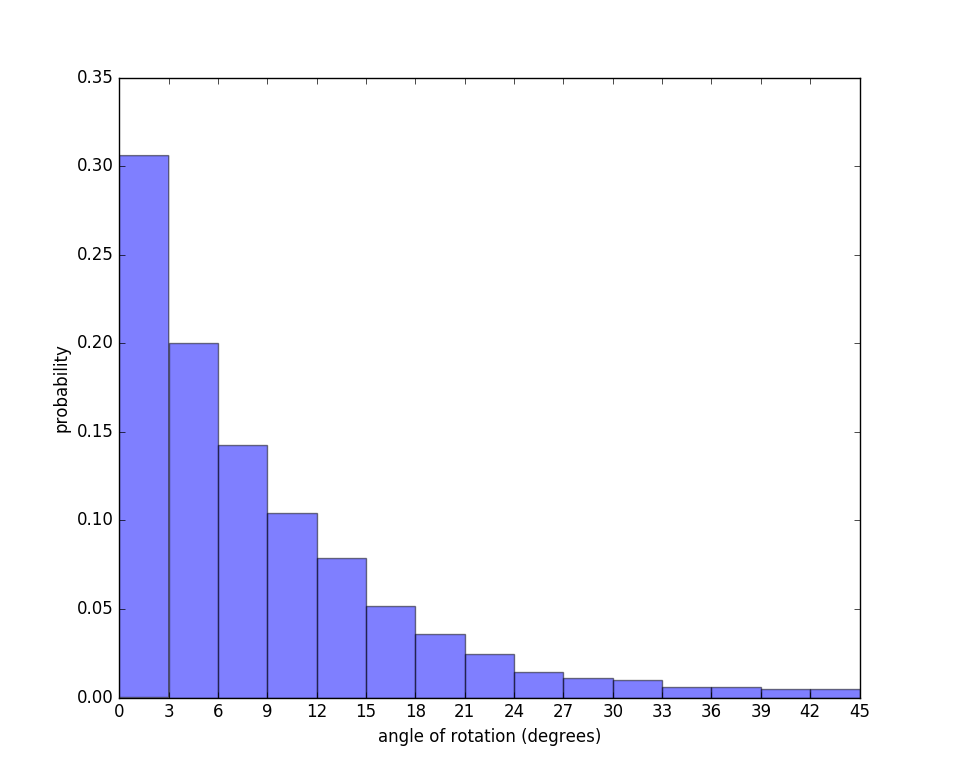
\includegraphics[width=\textwidth]{incidental_rotation.png}
	\caption{Angoli di rotazione delle bounding box in Incidental Text Scene.}
\end{figure}

\subsection{COCO Text}
\label{subsec:coco}
Introdotto nel 2016~\cite{cocotext} come estensione del MSCOCO Dataset, viene in seguito utilizzato per l'omonima competizione in occasione di ICDAR2017.
Punti di forza di questo dataset, oltre alla grande quantità di immagini, sono la varietà di contesti di acquisizione e la eterogeneità delle classi delle annotazioni. Per questo motivo lo si è scelto come base di training per i nostri esperimenti e come base per la validazione delle performance.\\
Non ci è possibile confrontarci con metodi concorrenti in quanto i risultati della competizione non sono ancora stati resi pubblici.\par
Caratteristiche:
\begin{itemize}
	\item
		$43.686$ immagini di training (118.309 parole)
	\item
		$10.000$ immagini di validation (27.550 parole)
	\item
		$10.000$ immagini di test
	\item
		groundtruth composta da bounding box ortogonali e trascrizione per ogni parola, ognuna con i seguenti attributi:
		\begin{itemize}
			\item
				machine printed / handwritten / altro
			\item
				leggibile / illeggibile
			\item
				inglese / non-inglese / sconosciuto
		\end{itemize}
\end{itemize}

\begin{figure}[H]
	\centering
	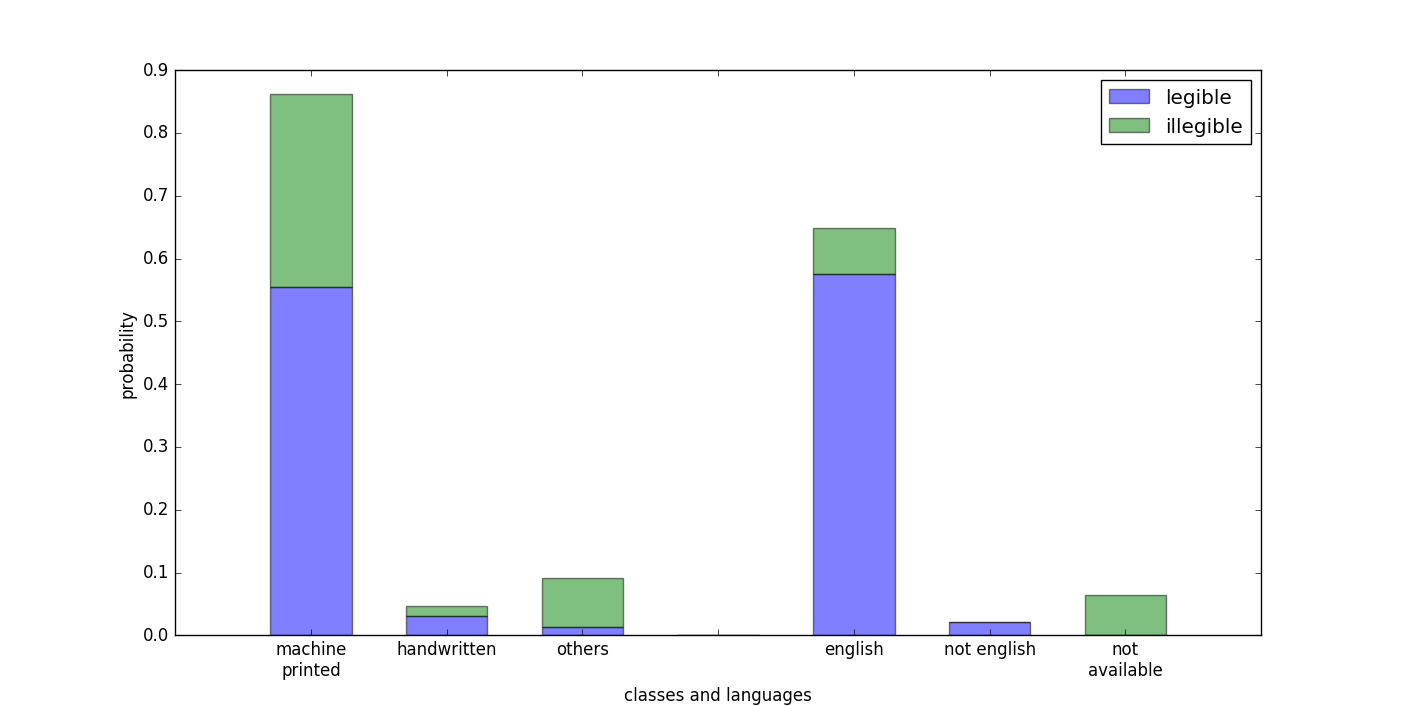
\includegraphics[width=1\textwidth]{annotation_classes_languages.png}
	\caption{Classificazione delle annotazioni}
\end{figure}

\subsection{SynthText}
\label{subsec:synth}
Introdotto nel 2016~\cite{synthtext}, ma mai utilizzato come base di training in nessuna competizione, la peculiarità di questo dataset risiede nel fatto che il testo è inserito sinteticamente, con una certa context-awareness, in immagini reali.\par
Caratteristiche:
\begin{itemize}
	\item
		$858.750$ immagini
	\item
		$7.266.866$ parole
	\item
		$28.971.487$ lettere
	\item
		groundtruth composta da trascrizioni e coordinate dei vertici delle bounding box orientate di ogni parola ed ogni singola lettera
\end{itemize}
\vfill
\begin{figure}[H]
	\centering
	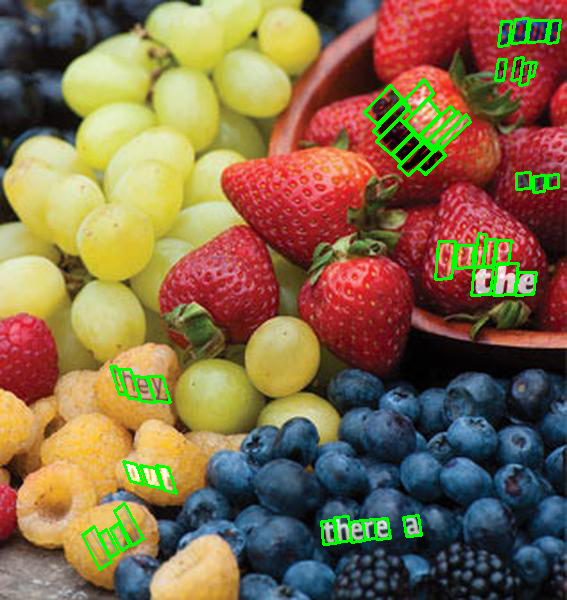
\includegraphics[width=0.7\textwidth]{synth_example.png}
	\caption{Immagine di training SynthText}
\end{figure}

\begin{figure}[H]
	\centering
	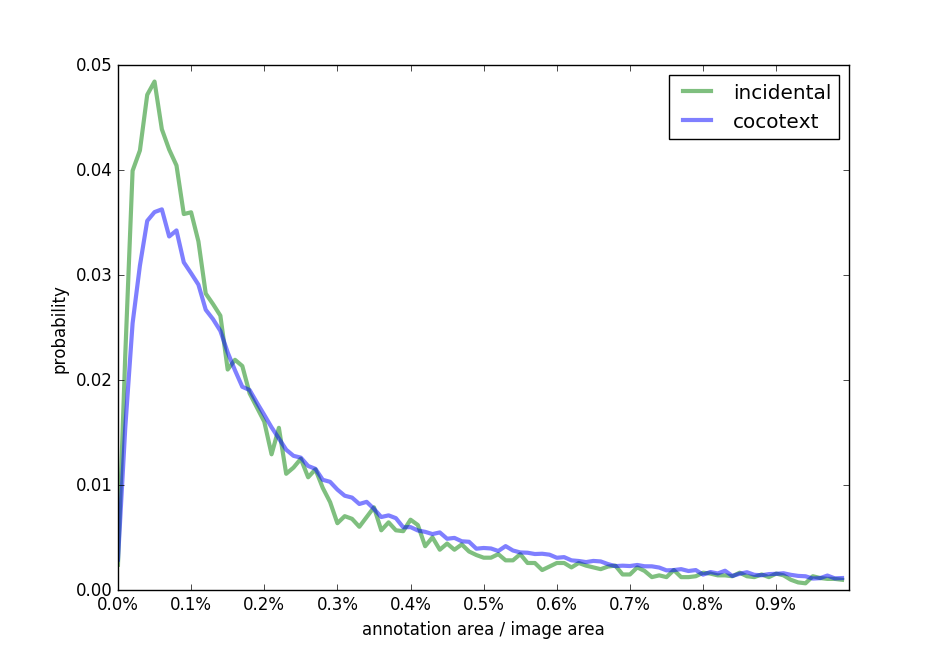
\includegraphics[width=\textwidth]{annotation_ratio.png}
	\caption{Area occupata dalle singole annotazioni nalle rispettive immagini}\label{fig:annratio}
	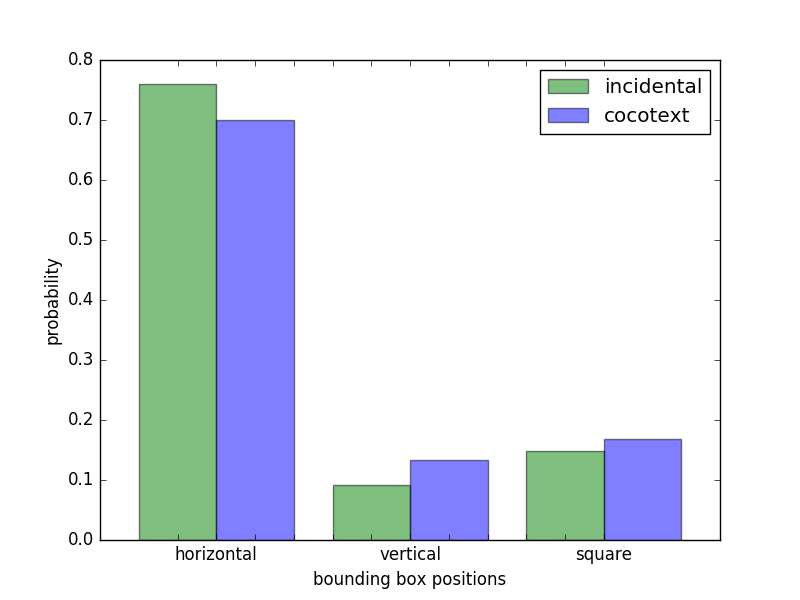
\includegraphics[width=0.9\textwidth]{annotation_position.png}
	\caption{Proporzioni delle upright bounding box}\label{fig:annprop}
\end{figure}



\section{Metodi di valutazione}
Come già precedentemente annoverato, per la comparazione tra metodi diversi che concorrono per lo stesso fine, si necessita di valori di riferimento omogenei e significativi.
In seguito verranno dunque illustrati più in dettaglio i vari metri di valutazione presenti in letteratura utilizzati per i nostri esperimenti e competizioni di riferimento.\par

\subsection{Precision \& Recall}
Quelle che seguono in questa sezione sono statistiche generali per la classificazione binaria indipendenti dallo specifico task.

\subsubsection{Precision}
Indica la percentuale di predizioni corrette rispetto al numero di predizioni totali.
Viene calcolata come segue:
$$
\text{precision} = \frac{\text{true positives}}{\text{true positives} + \text{false positives}} = \frac{tp}{n}
$$

\subsubsection{Recall}
Indica la percentuale di predizioni corrette rispetto al numero di istanze significative totali.
Viene calcolata come segue:
$$
\text{recall} = \frac{\text{true positives}}{\text{true positives} + \text{false negatives}}
$$

\subsubsection{F1-score}
Questa misura prende in considerazione entrambi i criteri precedentemente descritti calcolandone la media armonica, evitando perciò i problemi che potrebbero nascere dalla semplice media artimetica qualora la recall fosse molto bassa e la precision alta (poche predizioni ma corrette) e viceversa (molte predizioni fra cui molte erronee).
$$
F_{1} =
		\frac{2}{\frac{1}{\text{recall}} + \frac{1}{\text{precision}}}
	  =
		2 \cdot \frac{\text{precision} \cdot {\text{recall}}}{\text{precision} + \text{recall}}
$$

\subsubsection{Average Precision}
Anche questa stima utilizza sia la precision che la recall, ma in più necessita di un livello di confidenza per ogni predizione in modo da poter calcolare una curva di precision/recall dalla qualle estrarre l'area sottostante, il cui valore corrisponde alla precisione media. Quantizzata risulta calcolabile come:
$$
\sum_{k=1}^{N}{P(k) \Delta r(k)}
$$
dove $N$ è il numero totale di predizioni, $P(k)$ è la precisione al livello di confidenza $k$ e $\Delta r(k)$ è la differenza tra i valori di recall tra gli step di confidenza $k-1$ e $k$.

\subsection{Intersection over Union}
Se prima abbiamo visto metri di valutazione generici, quello qui descritto è invece specifico del campo dell'object detection.
Infatti poiché nei task di rilevamento risulta altamente improbabile predire un match esatto di una bounding box, è nata la necessità di uno standard di valutazione coerente ed efficace con il quale si potesse distinguire un \textit{vero positivo} da un \textit{falso positivo} influenzando di conseguenza tutte le misure descritte fin'ora.\par
Come suggerito dal nome, questa metrica è calcolata prendendo il rapporto tra l'area dell'intersezione e l'area dell'unione di due bounding box, predizione e groundtruth. Essendo il risultato un semplice valore numerico, è necessario porre una soglia per l'avvenuta detection, solitamente impostata a $0.5$ (oppure $0.75$ per valutazioni più meticolose).\par
Una delle caratteristiche principali dell'IoU è la penalizzazione dei casi in cui oggetti multipli appartenenti alla stessa classe vengano rilevati in una bounding box unica, ma specularmente si rischia di avere risultati ingannevoli nel caso in cui le annotazioni presentino errori o qualora il modello riesca addirittura a superare l'accuretezza della groundtruth.\par

\begin{figure}[H]
	\centering
	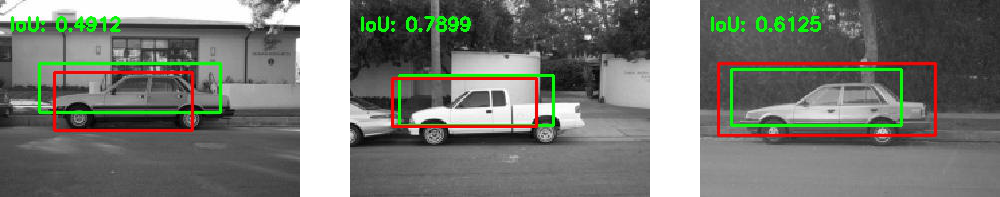
\includegraphics[width=\textwidth]{iou.png}
	\caption{Esempi di valutazione con IoU.}
\end{figure}


\chapter{Reti Neurali}

In questo capitolo verrà illustrato lo strumento principale utilizzato per lo sviluppo di un metodo di text localization, partendo dapprima dagli albori delle reti neurali, passando per i vari sviluppi negli anni nei vari campi, fino ad arrivare alla struttura alla base del nostro metodo.

\section{Reti Neurali Artificiali}

Le \textit{reti neurali artificali} possono essere definite come un modello matematico ispirato alle reti neurali biologiche, costituito da neuroni artificali interconnessi e da processi che dettano il cambiamento della propria struttura in base a informazioni che scorrono attraverso la rete durante la cosiddetta fase di apprendimento.

Il primo accenno al termine si deve a McCulloch e Pitts~\cite{McCulloch1943} che nel 1943 introdussero un combinatore lineare a soglia, esemplificato nella figura~\ref{fig:TLU}, in grado di ricreare funzioni booleane.

\begin{figure}[H]
	\centering
	\begin{equation*}
		\begin{aligned}[c]
			TLU(\vec{x}) &= \phi \bigg( \sum_{i=1}^{n}{w_{i} \cdot x_{i}} \bigg) \\
			\phi(x) &= x - \theta \geq 0
		\end{aligned}
		\quad
		\begin{aligned}[c]
			n &= 2 \\
			\theta &= 1.5 \\
		\end{aligned}
		\quad
		\begin{aligned}[c]
			w_{1} &= 1.0 \\
			w_{2} &= 1.0
		\end{aligned}
	\end{equation*}
	\caption{Threshold Logic Unit con relativi parametri per l'implementazione dell'and logico.}
\label{fig:TLU}
\end{figure}

Questo però non era che un semplice modello statico incapace di apprendere.
L'intuizione che diede vita ad una gran varietà d studi riguardando metodi di apprendimento automatico si deve infatti a D.O. Hebb~\cite{Hebb} il quale nel 1949 ipotizzò come l'apprendimento negli esseri viventi non fosse altro che un meccanismo di plasticità sinaptica, ovvero una modifica di intensità delle relazioni fra neuroni in base agli impulsi che li attraversano.

\subsection{Perceptron}
F. Rosenblatt ideò nel 1958 il \textit{Perceptron}\cite{rosenblatt1958perceptron}, un classificatore binario lineare, oggi considerato la più semplice rete neurale \textit{feed-forward}.

Il Perceptron può essere modellato come segue:
\begin{equation*}
	\begin{aligned}[c]
		y = f(x) =
			\begin{cases}
				1 &\text{se } w\vec{x} > 0 \\
				0 &\text{altrimenti}
			\end{cases}
	\end{aligned}
\end{equation*}

dove si incorpora un valore scalare di \textit{bias} con 
\begin{equation*}
	\begin{aligned}[c]
		w = \begin{bmatrix}
			w_{1} & \cdots & w_{d} & b
		\end{bmatrix}
	\end{aligned}
	\quad
	\begin{aligned}[c]
		\vec{x} = \begin{bmatrix}
			x_{1} \\
			\vdots \\
			x_{d} \\
			1
		\end{bmatrix}
	\end{aligned}
\end{equation*}

Si parte dunque da un dataset $D = \{(x^{(1)},g^{(1)}),\ldots, (x^{(n)},g^{(n)})\}$ formato da $n$ campioni $x^{(i)} \in \mathbb{R}^{d}$, vettori delle feature $d$-dimensionali, e $g^{(i)}$ valore di output desiderato per $f(x^{(i)})$. L'algoritmo è descritto di seguito:

\begin{enumerate}
	\item
		Inizializzazione del vettore $w$ con valori nulli o randomici tendenti a zero.
	\item
		Per ogni campione $i$ nel dataset $D$:
		\begin{enumerate}
			\item
				Calcolare $y$ al tempo corrente $t$: \\
				$y^{(i)}(t) = f[w(t) \cdot \vec{x}^{(i)}]$
			\item
				Aggiornare i valori di $w$ al nuovo tempo $t+1$: \\
				$\forall j \quad w_{j}(t+1) = w_{j}(t) + (g^{(i)} - y^{(i)}(t))x^{(i)}_{j}$
	\item
		Ripetere dal punto 2 per minimizzare $\frac{1}{n}\sum\limits_{i=1}^{n}|g^{(i)} - y^{(i)}(t)|$
		\end{enumerate}
\end{enumerate}

\subsection{Backpropagatin}
Dal 1969 la ricerca si bloccò con la dimostrazione da parte di Minsky e Papert~\cite{minsky1972} dell'impossibilità di risolvere problemi con soluzioni non separabili linearmente.
Negli anni a seguire le reti neurali vennero presto dimenticate a favore di altri modelli, come le Support Vector Machine, al tempo più efficaci nell'ambito del machine learning.\par
Nonostante questo nel 1975 venne introdotto da parte di Paul Werbos l'algoritmo per la cosiddetta \textit{backpropagation} il quale rimane tutt'oggi un ingranaggio principale per il funzionamento della gran parte delle reti neurali.

Sia $N$ una rete neurale con $e$ connessioni, $m$ input, $n$ output, $p$ osservazioni ed $E$ una funzione di costo da ottimizzare. Avremo dunque:
\begin{equation*}
	\begin{aligned}[c]
		x^{(1)},\dots,x^{(p)} \\
		y^{(1)},\dots,y^{(p)} \\
		w^{(0)},\dots,w^{(p)} \\
	\end{aligned}
	\quad
	\left.\begin{aligned}[c]
		\text{vettori di input in } &\mathbb{R}^m \\
		\text{vettori di output in } &\mathbb{R}^n \\
		\text{vettori dei pesi in } &\mathbb{R}^e
	\end{aligned}\quad \right\}
	\;
	\begin{aligned}[c]
		&y &=& &f_{N}(x,w) \\
		&E &\colon& &\mathbb{R}^{n \times n} \rightarrow \mathbb{R}
	\end{aligned}
\end{equation*}

L'output dell'algoritmo è dato da un nuovo vettore dei pesi ottenuto con il metodo del gradiente, calcolato di conseguenza dalla derivata della funzione di costo rispetto a $w$:
$$
\frac{d E}{d w}
$$

Per una serie di input perciò, partendo dal vettore $w^{(0)}$ inizializzato con valori prossimi a zero, si calcola $E(y^{(i)}, f(x^{(i)}, w^{(i-1)}))$ iterativamente ponendo $w^{(i)}$ uguale all'output dell'algoritmo alla fine di ogni iterazione.

\subsection{Multilayer Perceptron}
\label{subsec:mlp}

Partendo dai concetti precedentemente presentati passeremo ora a mostrare come costruire una semplice rete neurale artificiale con la relativa fase di addestramento: il \textit{Multilayer Perceptron}.\par
Esso è così chiamato in quanto non è altro che un'estensione del Perceptron che può essere visto come una rete neurale con $d$ neuroni in entrata (rappresentanti il vettore $x \in \mathbb{R}^d$) ed un singolo neurone in uscita, con le connessioni rappresentate dalla funzione $f(x)$.\par

Nel Multilayer Perceptron questa struttura viene ampliata aggiungendo almeno uno \textit{strato nascosto} tra il layer di input e quello di output formato da un numero arbitrario di neuroni.
Ciò che si viene a creare è dunque un grafo diretto aciclico, come mostrato in figura~\ref{fig:MLP}, in cui i neuroni appartenenti allo stesso layer non sono connessi fra di loro.

\begin{figure}[H]
	\centering
	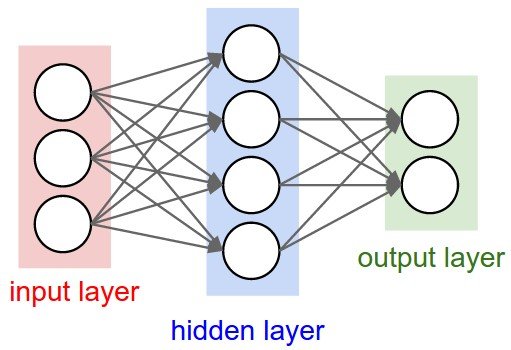
\includegraphics[width=0.4\textwidth]{neural_net.jpeg}
	\caption{Rappresentazione grafica di un Multilayer Perceptron}
\label{fig:MLP}
\end{figure}

Le connessioni fra due strati $x$ e $y$ di $n$ e $m$ neuroni rispettivamente, possono essere formalizzate come segue:

\begin{equation*}
	\left.\begin{aligned}[c]
		x &\in \mathbb{R}^{n \times 1} &\quad 
		y &\in \mathbb{R}^{m \times 1} \\
		W &\in \mathbb{R}^{m \times n} &\quad
		b &\in \mathbb{R}^{m \times 1} \\
	\end{aligned}\quad \right\}
	\;
	\begin{aligned}[c]
		y = \phi(Wx + b)
	\end{aligned}
\end{equation*}

Altra aggiunta che si può notare nella formalizzazione è la presenza di $\phi$ ovvero una funzione di attivazione che aggiunge non linearità al modello multistrato e permette alla rete di approssimare qualsiasi funzione, come dimostrato nel 1989 da Cybenko\cite{Cybenko1989}.
Le funzioni di attivazione, illustrate nella figura~\ref{fig:ACT}, possono essere di vario tipo, di seguito sono elencate le più importanti:

\begin{description}[leftmargin=!,labelwidth=\widthof{\bfseries Exponential Linear Unit (ELU)}]
\label{itm:relus}
	\item[Funzione Logistica] 
		${(1 + e^{-x})}^{-1}$
	\item[Tangente Iperbolica]
		$\tanh(x)$
	\item[Rectified Linear Unit (ReLU)]
		$\max(0,\, x)$
	\item[Leaky ReLU]
		$\max(0.01x,\, x)$
	\item[LReLU Parametrica]
		$\begin{cases}
			\alpha x &\text{se } x \geq 0 \\
			x &\text{se } x < 0 \\
		\end{cases}$
	\item[Exponential Linear Unit (ELU)]
		$\begin{cases}
			\alpha(e^x - 1) &\text{se } x \geq 0 \\
			x &\text{se } x < 0 \\
		\end{cases}$
\end{description}

\begin{figure}[H]
	\centering
	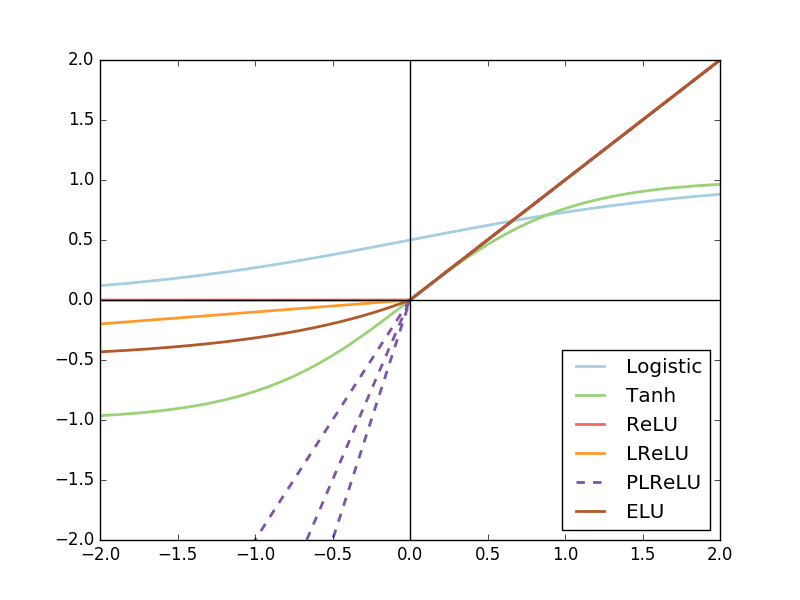
\includegraphics[width=0.6\textwidth]{activation_function.png}
	\caption{Comparazione fra le diverse funzioni di attivazione.}
\label{fig:ACT}
\end{figure}


Dato il modello appena descritto dunque non rimane che utilizzarlo come classificatore (con più di due classi e non-lineare a differenza del Perceptron di base) oppure per un task di regressione. Il prossimo passo è perciò quello di definire la funzione di costo (detta in gergo di \textit{Loss}) da utilizzare con l'algoritmo di backpropagation.


\subsection{Funzioni di Loss}

\subsubsection{Classificazione}
Assumiamo che ogni neurone $f_{j}$ del layer di output rappresenti uno score di appartenenza ad un certa classe e $y$ sia la classe a cui appartiene $x$:
\begin{description}
	\item[Hinge Loss]
		\quad\\$\Delta$ rappresenta la distanza minima richiesta di ogni score da quello della classe corretta.
		$$
		L = \sum_{j \neq{} y}{\max(0,\, {f_j} -{f_y} +\Delta)}
		$$
	\item[Softmax Cross-Entropy]
		\quad\\Con questo metodo lo score di ogni classe viene normalizzato. Il valore di loss finale è tanto minore quanto vicino a $1$ è la probabilità della classe corretta.
		$$
		L = -\log{\bigg(\frac{e^{f_y}}{\sum_j{e^{f_j}}}\bigg)}
		$$
\end{description}


\subsubsection{Regressione}
Assumiamo che ogni neurone $f_{i}$ del layer di output rappresenti una quantità da predire e $y$ sia un vettore dei valori attesi.

\begin{description}
	\item[L1 Loss]
		\quad\\Distanza di Manhattan.
		$$
		L = \Vert{f-y}\Vert_1 = \sum_{i}{\mid{f_i -y_i \mid}}
		$$
	\item[L2 Loss]
		\quad\\Distanza euclidea al quadrato per facilitare il calcolo della derivata durante la backpropagation.
		$$
		L = \Vert{f -y \Vert_2^2} = \sum_{i}{ (f_i -y_i)^2 }
		$$
\end{description}


\subsection{Apprendimento}

Ultimo passo per completare il meccanismo di apprendimento di una rete neurale è quello di definire come l'algoritmo di backpropagation dovrà aggiornare i valori dei vari neuroni.

Il metodo base della discesa stocastica del gradiente (SGD) opera come segue su un certo vettore $x$ di parametri al tempo $t+1$ utilizzando un \textit{learning rate} $\eta$ predefinito:
$$
x_{t+1} = x_t -\eta{} \cdot \frac{dL}{dx_t}
$$

In seguito verranno elencate diverse ottimizzazioni da poter usare insieme al metodo di base per accellerare il processo di apprendimento.\\
Ci riferiremo ai gradienti calcolati più semplicemente con:
$$dx_t = \frac{dL}{dx_t}$$

\subsubsection{Momentum Update}\cite{Momentum}
Viene aggiunto un ulteriore iperparametro $\alpha$ e una variabile $\Delta{x}$ in maniera da favorire la discesa in punti con alto gradiente.
\begin{align*}
	\Delta x_{t+1} &= \eta \cdot dx_t + \alpha \Delta x_t \\
	x_{t+1} &= x_t - \Delta x_{t+1}
\end{align*}

\subsubsection{Adagrad}\cite{Adagrad}
Learning rate adattivo per ogni singolo parametro grazie ad una variabile che tiene traccia del quadrato del gradiente.
\begin{align*}
	G_{x}^{(t+1)} &= G_x^{t} + dx_t^2 \\
	x_{t+1} &= x_t - \frac{\eta \cdot dx_t}{\sqrt{G_x^{(t+1)}} + \epsilon}
\end{align*}
\subsubsection{RMSProp}\cite{RMSProp}
Simile ad Adagrad con l'aggiunta di un iperparametro $\beta$ (decay rate) che previene la descrescenza monotonica del learning rate mantenendo una media mobile del quadrato del gradiente.
\begin{align*}
	G_x^{(t+1)} &= \beta \cdot G_x^t + (1 - \beta) \cdot dx_t^2 \\
	x_{t+1} &= x_t - \frac{\eta \cdot dx_t}{\sqrt{G_x^{(t+1)}} + \epsilon}
\end{align*}
\subsubsection{Adam}\cite{Adam}
Utilizza le medie mobili sia del gradiente che del suo quadrato introducendo dunque due iperparametri $\beta_1$ e $\beta_2$. Queste vengono in seguito corretti per evitare un annichilimento durante le prime iterazioni. 
\begin{align*}
	m_x^{(t+1)} &= \beta_1 \cdot m_t + (1-\beta_1) \cdot dx_t \quad&
	\hat{m}_x &= \frac{m_x^{(t+1)}}{1 - \beta_1^t} \\
	v_x^{(t+1)} &= \beta_2 \cdot v_t + (1-\beta_2) \cdot dx_t^2 \quad&
	\hat{v}_x &= \frac{m_x^{(t+1)}}{1 - \beta_2^t}
\end{align*}
$$
  x_{t+1} = x_t - \frac{\eta \cdot \hat{m}_x}{\sqrt{\hat{v}_x} + \epsilon}
$$

\subsection{Ottimizzazioni}

In questa sezione verranno discussi i principali metodi che consentono il miglioramento delle prestazioni di una qualsiasi rete neurale, sia dal punto di vista della velocità che della qualità dell'apprendimento.

\subsubsection{Data preprocessing}

Le principali operazioni sono quelle di sottrazione del \textit{valore medio} dall'intero campione di dati di training e la sua \textit{normalizzazione} attraverso la divisione per la deviazione standard. Queste operazioni permettono di avere dei dati geometricamente centrati all'origine e con valori compresi tra -1 e 1.


\subsubsection{Dropout}

Introdotto nel 2014\cite{dropout}, consiste nell'introdurre una probabilità $p$ che ogni neurone ha di rimanere attivo durante la fase di addestramento. L'obiettivo è quello di evitare l'overfitting dei dati attraverso epoche diverse.

\begin{figure}[H]
	\centering
	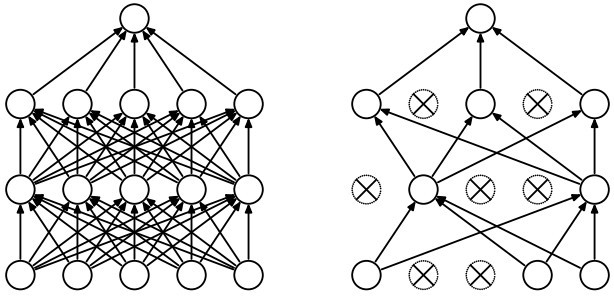
\includegraphics[width=0.6\textwidth]{dropout.jpeg}
	\caption{Rete neurale prima e dopo l'applicazione del dropout.}
\label{fig:dropout}
\end{figure}



\subsubsection{Inizializzazione dei pesi}

Dato che un'inizializzazione costante di tutti i pesi porterebbe a gradienti costanti, una soluzione consiste nell'utilizzare valori randomici prossimi a 0 distribuiti secondo una normale divisi per la radice quadrata del numero di input del layer. Ciò è dovuto dal fatto che un numero maggiore porterebbe ad una varianza sempre maggiore.
Dato però l'utilizzo di funzioni di attivazione, viene violata l'assunzione di una media nulla ed è dunque stata identificato il valore $\sqrt{2/n}$ come reale valore della varianza~\cite{he2015delving}.


\subsubsection{Batch Normalization}

Introdotta nel 2015\cite{batchnorm} con l'obiettivo di contrastare inizializzazioni sfavorevoli dei pesi nella rete, consiste nell'inserimento di un layer di normalizzazione tra ogni componente connessa e la relativa funzione di attivazione.


\section{Reti Neurali Convoluzionali}

Il modello di rete neurale visto fino ad ora rappresenta solamente le fondamenta degli strumenti odierni.
In seguito verranno dunque descritte le cosiddette \textit{CNN} in quanto modello principale che ha preso piede nel campo della Computer Vision.

\subsection{Struttura delle CNN}

Prima di illustrare le varie architetture che si son succedute negli anni è doveroso spiegare come si possa adattare un modello basato su \textit{fully-connected layers} (come per il Multilayer Perceptron visto nella sezione~\ref{subsec:mlp}) in modo da avere come input delle immagini (anche di dimensione diversa) evitando l'esplosione del numero di pesi da addestrare.

\subsubsection{Convolution Layer}
Ovvero il layer principale che dà il nome alle reti neurali convoluzionali.
L'idea principale è quella di avere $n$ filtri, solitamente di 3 o 5 pixel per lato, che vengono applicati all'input.
Gli iperparametri principali sono:
\begin{itemize}
	\item \textbf{Dimensione} del filtro.
	\item \textbf{Profondità}, il numero di filtri.
	\item \textbf{Stride}, di quanti pixel spostare il filtro.
	\item \textbf{Padding}, se aggiungere un bordo all'input per mantenere costante la dimensioni in output e nel caso quali valori usare.
\end{itemize}
\vspace{\fill}
\begin{figure}[H]
	\centering
	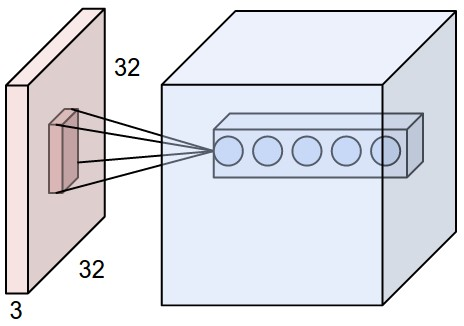
\includegraphics[width=0.4\textwidth]{convlayer.jpeg}
	\caption{Visualizzazione di un'operazione di convoluzione.}
\label{fig:convlayer}
\end{figure}

\subsubsection{ReLU Layer}
Applicazione delle funzioni di attivazione descritte nella sezione~\ref{itm:relus}.

\subsubsection{Pooling Layer}
Consente di ridurre la dimensione spaziale dell'input in base ad iperparametri $s$ stride e $n$ estensione del campo ricettivo.\\
I criteri di scelta del valore di output sono principalmente due: \textit{max pooling} (scelta del massimo) oppure \textit{average pooling} (scelta della media).\par

\subsubsection{Deconvolution Layer}
Non è altro che una convoluzione con stride frazionario che aumenta le dimensioni spaziali (de-pooling) dell'input ma che ne riduce la profondità invertendo dunque il \textit{forward pass} con il \textit{backward pass}.


\subsection{Breve storia}

\subsubsection{LeNet}

Nonostante già nel 1988~\cite{zhang1990parallel} vennero mossi i primi passi verso l'ideazione di un precursore delle reti convoluzionali, solo l'architettura ideata nel 1998 da LeCun et al.\cite{LeNet} viene oggi considerata come la prima vera \textit{CNN}.\par
Questo modello, introdotto con lo scopo di riconoscere caratteri scritti a mano, come mostrato in figura~\ref{fig:lenet5}, era composto da 4 sequenze di convoluzioni e ridimensionamenti, seguiti da 3 fully-connected layer ed una funzione a base radiale gaussiana finale per stimare gli errori per le singole classi.\par

\begin{figure}[H]
	\centering
	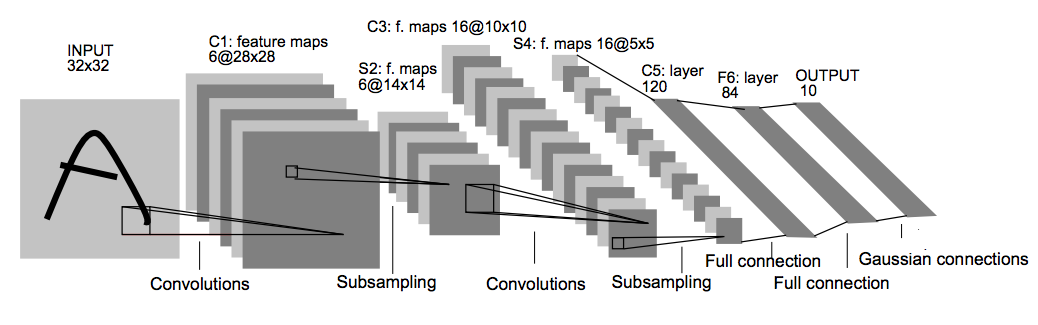
\includegraphics[width=0.9\textwidth]{lenet5.png}
	\caption{Schema di LeNet-5.}
\label{fig:lenet5}
\end{figure}

\subsubsection{GPGPU}
Questi sviluppi furono ancora osteggiati dall'elevata capacità computazionale richiesta per l'addestramento delle reti neurali. Nei primi anni del nuovo millennio infatti gli studi si concentrarono principalmente sullo studio di tecniche di addestramento attraverso l'utilizzo di \textit{Graphic Compute Units} in seguito alla pubblicazione di una ricerca nel 2005 che ne descriveva il loro valore nel campo del machine learning.\cite{gpuml}

\subsection{Casi di studio}
\label{subsec:case_studies}
Di seguito descriveremo velocemente diverse architetture sviluppatosi molto recentemente in seguito all'implementazione di LeNet su GPU nel 2011.\cite{gpu2011}

\subsubsection{AlexNet}
Questa rete neurale\cite{alexnet} è presentata in occasione della \textit{ImageNet ILSVRC Challenge}\cite{ILSVRC15} nel 2012, competizione annuale che prevedeva task di classificazione e localizzazione di ben 1000 classi differenti. Prendendo spunto direttamente da LeNet, questa architettura è riuscita a raggiungere risultati inimmaginabili sovraperformando il secondo classificato di ben 10 punti sulla percentuale d'errore.
\vfill
\begin{figure}[H]
	\centering
	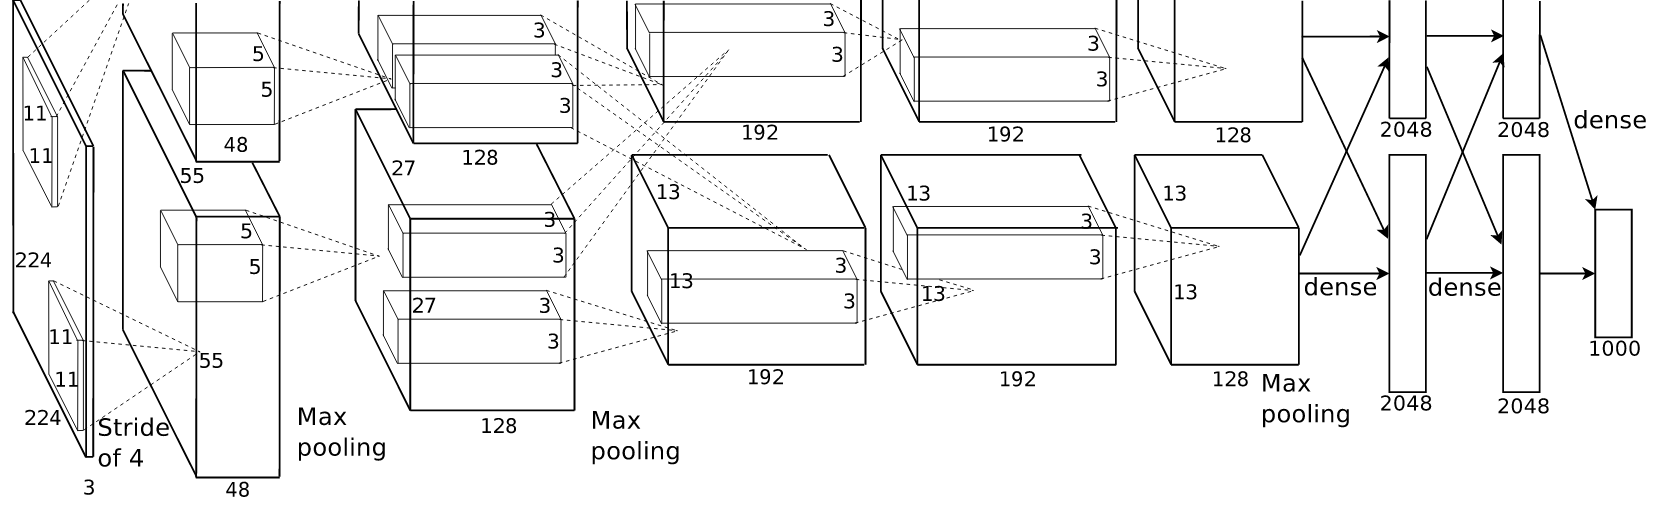
\includegraphics[width=\textwidth]{alexnet.png}
	\caption{Schema di AlexNet.}
\label{fig:alexnet}
\end{figure}
\vfill
\subsubsection{GoogLeNet}
Vincitrice dela \textit{ImageNet ILSVRC Challenge} nel 2014, ideata da Szegedy et al.\ da Google~\cite{googlenet}, ha introdotto il concetto di \textit{Inception Module}, illustrato in figura~\ref{fig:inception}, in maniera da ridurre drasticamente il numero di parametri (4 milioni rispetto ai 60 di AlexNet).

\begin{figure}[H]
	\centering
	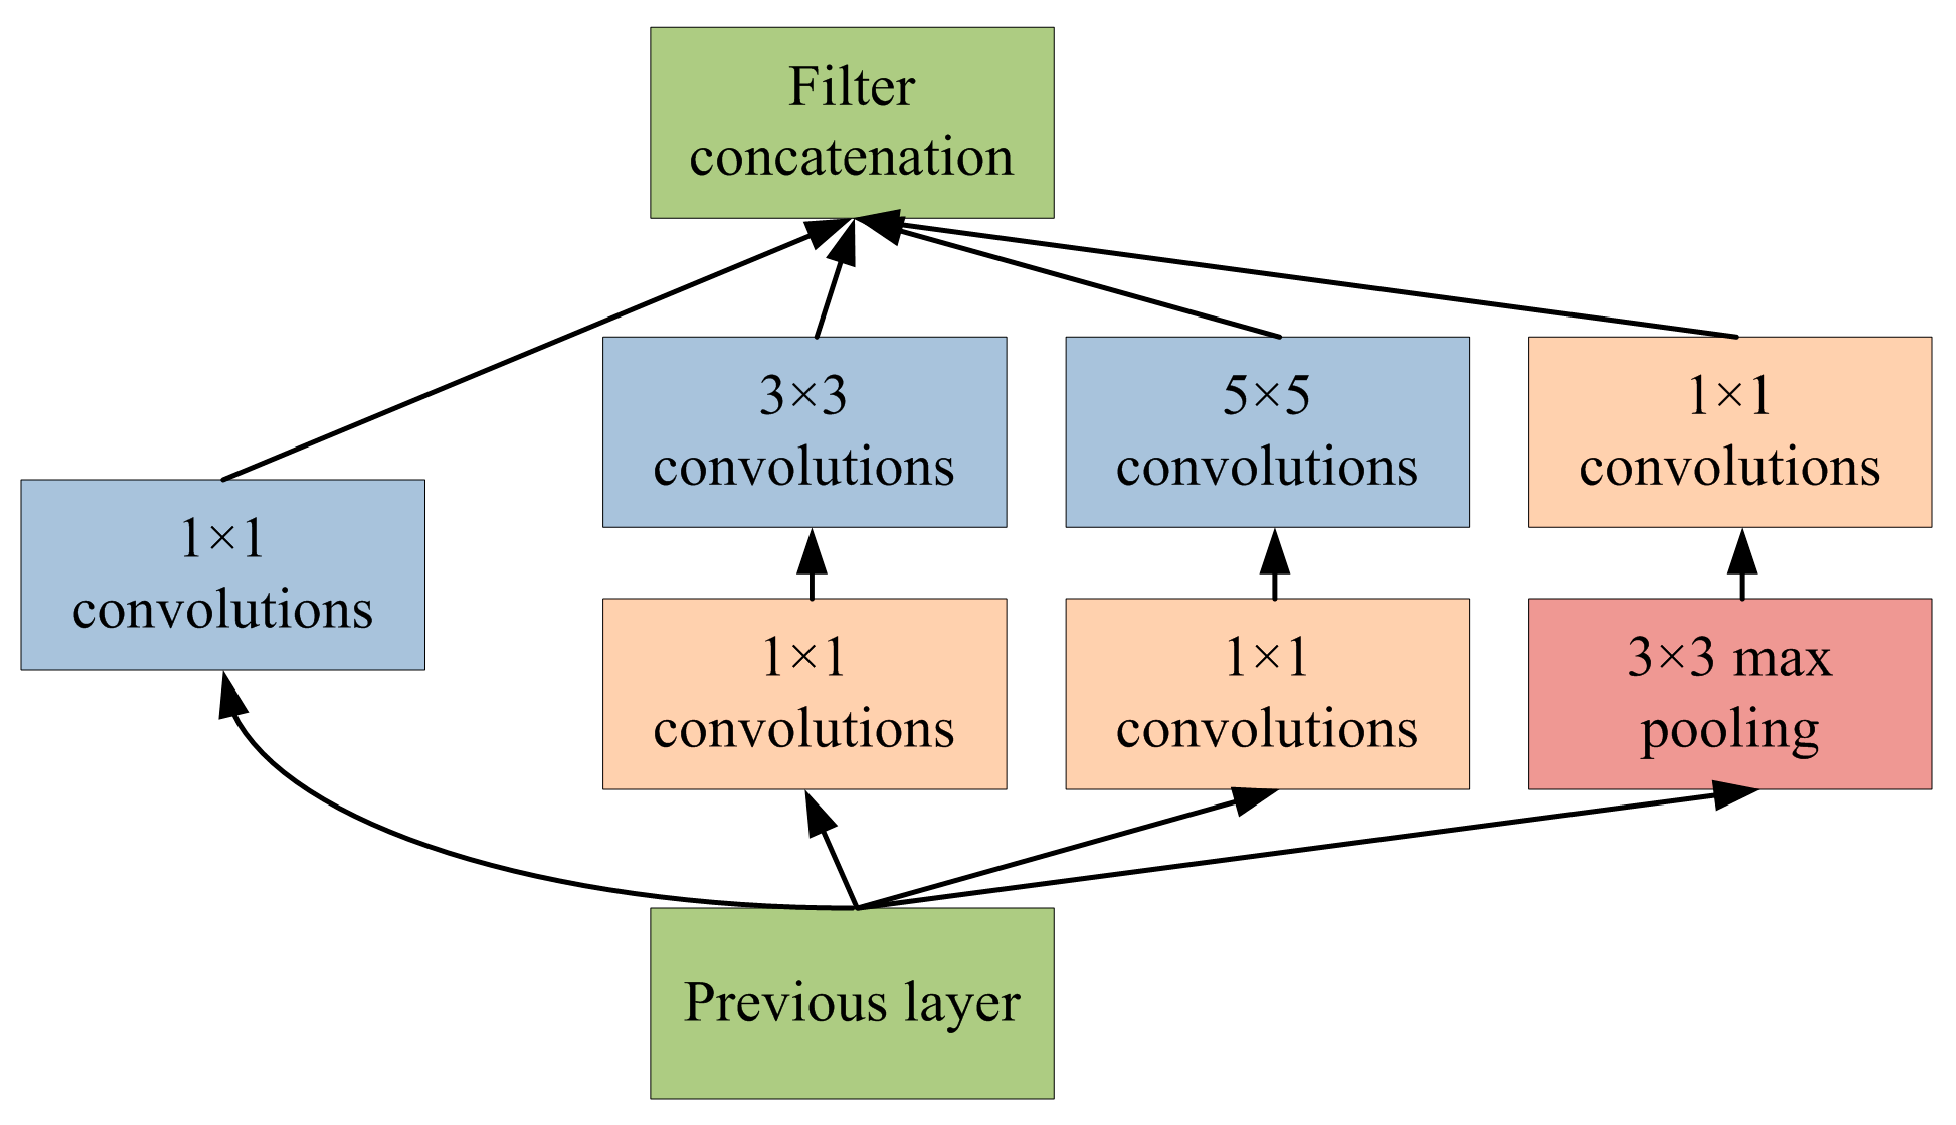
\includegraphics[width=0.6\textwidth]{inception_module.png}
	\caption{Inception Module di GoogLeNet.}
\label{fig:inception}
\end{figure}

\subsubsection{VGG}
Nonostante si è classificata solo in seconda posizione scontrandosi con GoogLeNet, questa architettura ideata da Karen Simonyan and Andrew Zisserman\cite{VGG} ha mostrato che la \textit{profondità} di una rete era una componenete principale per performance maggiori. Altro punto di forza è la sua semplicità strutturale nonostante il numero di parametri elevato, ben 140 milioni, dovuti agli ultimi fully-connected layer.
\begin{figure}[H]
	\centering
	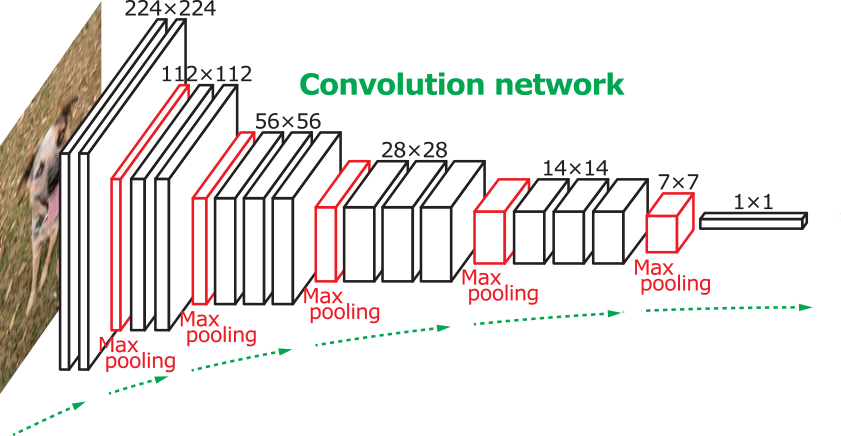
\includegraphics[width=0.75\textwidth]{vgg16.png}
	\caption{Schema di VGG16.}
\label{fig:vgg16}
\end{figure}

\subsubsection{ResNet}
\cite{resnet}Vincitrice di \textit{ILSVRC Challenge 2015}, introduce le cosiddette \textit{Shortcut Connections}, illustrate in figura~\ref{fig:residual}, in modo da risolvere il problema della degradazione del segnale di errore in reti molto profonde.

\begin{figure}[H]
	\centering
	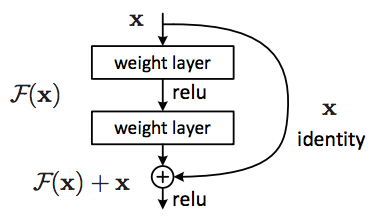
\includegraphics[width=0.5\textwidth]{residual_block.png}
	\caption{Shortcut Connection.}
\label{fig:residual}
\end{figure}


\section{Fully Convolutional Network}
\label{sec:FCN}
Tutte le architetture citate in precedenza per quanto potenti ed innovative, nella loro configurazione di base sono solo atte a classificare un'immagine, ovvero a fornire le probabilità di appartenenza a ciascuna classe su cui sono state addestrate.\par
Questa limitazione perciò non ci permette di eseguire classificazioni multiple o localizzazioni, per esempio separare due oggetti appartenenti alla stessa classe oppure rilevare due oggetti di due classi differenti all'interno di una stessa immagine.\par
Per la localizzazione singola di una classe una soluzione banale è quella di passare da un task di classificazione ad uno di regressione delle coordinate della bounding box cambiando dunque la funzione di loss finale.\par
Negli anni si sono avuti ulteriori raffinamenti atti a compensare queste lacune, dapprima con FastRCNN\cite{fastrcnn} ed il successivo FasterRCNN\cite{fasterrcnn} e più recentemente con YOLO\cite{yolo}, tutti nati con lo scopo di predire bounding box multiple con rispettive classi di appartenenza. Quello però di cui tratteremo in questa sezione è un approccio completamente differente.\par
Ideata nel 2014~\cite{fcn}, una \textit{Fully Convolutional Network} si pone l'obiettivo di generare un output della stessa dimensione dell'immagine di input in cui ogni pixel rappresenta la propria classe di appartenenza, praticamente semgentando l'immagine originale.\par
Grande pregio di questa architettura è la propria semplicità strutturale, infatti, come mostrato in figura~\ref{fig:fcn}, non fa altro che riprendere la \textit{VGG16} ed ampliarla aggiungendo uno o più layer di deconvoluzione addizionati ai precedenti output dei layer di pooling per generare l'immagine finale.

\begin{figure}[H]
	\centering
	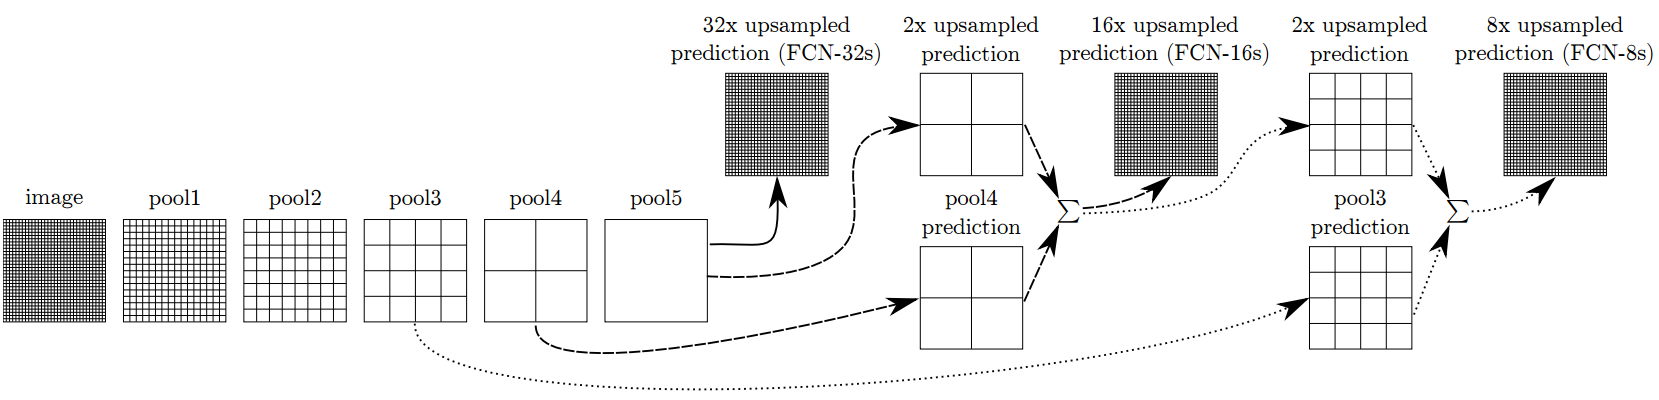
\includegraphics[width=\textwidth]{fcn.png}
	\caption{Schema delle Fully Convolutional Network.}
\label{fig:fcn}
\end{figure}


\chapter{Esperimenti}

Per il perseguimento dello scopo di questa tesi si è deciso  di utilizzare un approccio con reti neurali convoluzionali basato sull'architettura delle Fully Convolutional Networks esposte nel capitolo precedente. Verranno dunque qui mostrate le motivazioni di questa scelta, l'evoluzione del metodo sviluppato e varie considerazioni sui risultati ottenuti.

\section{Descrizione del metodo}
Recentemente, come già accennato, l'architettura delle FCN si è dimostrata un mezzo potente per il rilevamento di oggetti nelle immagini, rendendo superflua la fase di \textit{region proposal} e ponendo in ombra metodi per la localizzazione multipla basati su RRCN.\par
È naturale quindi porsi la domanda di dove può arrivare la potenza di queste reti per task diversi da quelli per cui sono state concepite, ricordando che alla base vi è un generico classificatore.\par
Il nostro obiettivo è quello di trovare aree di testo in immagini digitali, quindi qualcosa che va al di là della semplice concezione di \textit{oggetto}. Un testo può infatti essere presente su una varietà immensa di oggetti eterogenei, basti pensare ai cartelli stradali, ai giornali, alle magliette oppure agli schermi di televisori e smartphone.\par
Pare dunque impossile definire un oggetto singolo classificabile come testo, se non pensando di isolare singolo carattare, obiettivo che ci viene reso impossibile dall'indisponibilità di un dataset adeguato.\par
Nonostante tutto, invece questa concezione astratta può venire superata dalle reti neurali attraverso un corretto addestramento date le giuste informazioni. A prova di ciò possiamo citare~\cite{pixellevel}, dove per localizzare le singole istanze di vari oggetti vengono utilizzate due FCN aggiuntive, una per la predizione della profondità e l'altra per la direzione dal centroide di ogni istanza. Si veda l'immagine~\ref{fig:pixellevel} per un'esempio della groundtruth.

\begin{figure}[H]
	\centering
	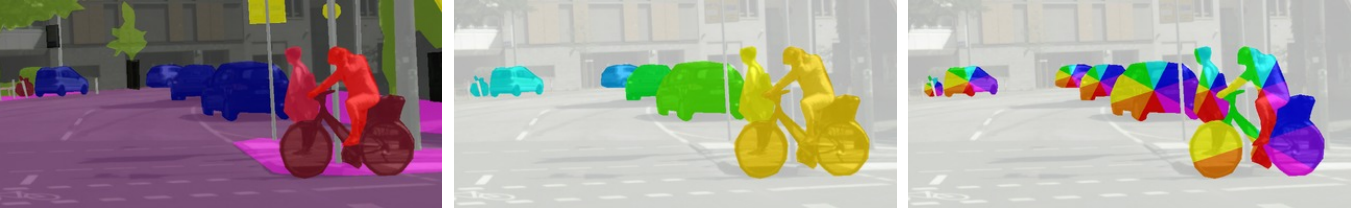
\includegraphics[width=\textwidth]{pixellevel.png}
	\caption{Esempi delle groundtruth.}
\label{fig:pixellevel}
\end{figure}

I più che discreti risultati di questo lavoro ci dimostrano dunque la grande versatilità di una FCN per un grade campo di mansioni che esulano da quello della loro concezione originale.

Assodato il fatto che verrà utilizzata una FCN per la segmentazione di un'immagine in area di testo e non, di seguito verrà descritto il processo di sviluppo della nostra pipeline per la localizzazione per poi confrontarci con metodi concorrenti.


\subsection{Strumenti}
Python\cite{python} si è imposto negli anni come linguaggio molto semplice da usare per la prototipizzazione di algoritmi nonostante la sua lentezza dovuta alla sua natura di linguaggio interpretato. Questa sua debolezza è però stata in parte superata grazie a moduli sviluppati come \textit{wrapper} intorno a librerie scritte in linguaggi compilati come C/C++, rendendo dunque più accessibile e semplificato l'utilizzo di routine altamente efficenti.\par
Tra le più famose, ed utilizzate in questa tesi, citiamo \textbf{NumPy}\cite{numpy} per la manipolazione di array multidimensionali, \textbf{SciPy}\cite{scipy} per gli algoritmi matematici più vari, \textbf{OpenCV}\cite{opencv} per l'elaborazione di immagini ed infine \textbf{Shapely}\cite{shapely} per la manipolazione di oggetti geometrici.\par
Per l'implementazione della \textit{Fully Convolutional Network} però ci si è affidati a \textbf{TensorFlow}\cite{tensorflow}, una libreria per l'implementazione, visualizzazione e profilazione di reti neurali sviluppata da Google dal 2015.


\subsection{Groundtruth}
%La definizione di una groundtruth è una fase estremamente importante in quanto da questa dipende tutto il processo di addestramento del nostro modello e l'estrapolazione finale dei dati a noi rilevanti.\par
L'output desiderato della nostra rete consiste in un'immagine delle stesse dimensioni di quella di input segmentata in due classi: testo e ``non testo'', quindi come prima idea potrebbe sovvenire quella di specificare, lettera per lettera, le aree di testo rispetto al background. Ciò potrebbe sembrare l'approccio migliore atto a generare risultati accuratissimi non solo per la localizzazione, ma anche per la segmentazione delle singole lettere per il successivo task di riconoscimento del testo, ma ad oggi non esistono dataset simili a nostra disposizione.\par
Il passo successivo è quindi quello di generalizzare l'idea precedente portando l'area di interesse non quindi alla forma della singola lettera, ma la sua posizione. Il dataset SynthText introdotto nella sezione~\ref{subsec:synth} viene in nostro soccorso, essendo infatti un dataset sintetico ci mette a disposizione questi dati specifici fornendo le bounding box per ogni carattere.\par
Per quanto riguarda gli altri dataset introdotti in precedenza, le loro annotazioni ci forniscono solo i dati approssimativi di una bounding box per parola, quindi possiamo ancora astrarre e considerare quelle zone come area di interesse, seppur aggiungendo teoricamente molto più rumore.\par


\subsection{Iperparametri}
La scelta di iperparametri per l'ottimizzazione di una rete neurale è una delle sfide maggiori che si affrontano durante la fase di addestramento di un modello. Di seguito sono elencati quelli principali individuati durante le fasi preliminari di preparazione della rete:
\begin{description}
	\item[Batch size:]
		Un numero maggiore velocizza l'apprendimento. $16$ è il massimo che si è potuto raggiungere rimanendo nei limiti di memoria a disposizione.
	\item[Learning rate:]
		Influenzato dal batch size, nonostante l'utilizzo di algoritmi sofisticati per la discesa del gradiente, valori troppo grandi ($10^{-4}$) non portano a nessuna predizione, mentre valori troppo piccoli ($10^{-6}$) rallentano l'apprendimento. $10^{-5}$ è il valore utilizzato per tutti gli esperimenti a seguire con Adam.
	\item[Loss function:]
		Pixelwise Softmax Cross-Entropy con azzeramento del valore di loss su zone con testo contrassegnato come illeggibile dai dataset in uso.
\end{description}


\subsection{Dettagli preliminari}

Prima di procedere con l'analisi dei vari esperimenti svolti è necessario chiarire alcuni punti riguardanti implementazione della rete, gestione dell'apprendimento, estrazione delle predizioni finali e utilizzo dei vari dataset.\par

\subsubsection{FCN}
\label{subsec:impl}
Qui elencate le caratteristiche principali dell'architettura: 
\begin{itemize}
	\item \textit{FCN-8} (3 deconvoluzioni con addizione di due layer di pooling come illustrato in figura~\ref{fig:fcn})
	\item \textit{VGG19} come classificatore con pesi già addestrati per ImageNet~\cite{pretrained}
	\item \textit{ReLU} standard
	\item \textit{Max Pooling}
	\item \textit{Padding} nell'ultima convoluzione della VGG per facilitare l'utilizzo della rete neurale su immagini di dimensione variabile
\end{itemize}


\subsubsection{Generazione dati di training}
\label{subsubsec:gendata}
Poiché le immagini dei vari dataset presentano risoluzioni pressoché sempre differenti, è necessario definire un metodo per ottenere zone di grandezza fissa da ciascuna di esse in modo da adoperare un batch size maggiore di 1.\par
L'idea di estrarre una zona randomica, seppur molto semplice, potrebbe rallentare l'addestramento in quanto, come già analizzato in figura~\ref{fig:annratio}, le zone di testo occupano un'area decisamente esigua rispetto all'immagine in cui compaiono, abbassando dunque le probabilità che possano essere incluse nel nostro ``ritaglio'' randomico.\par
La soluzione adottata consiste dunque nel partire da un'annotazione contrassegnata come leggibile e da lì espandere randomica la selezione verso i bordi dell'immagine, squadrarla (anche uscendo dai limiti) ed infine ridimensionare l'area selezionata alla risoluzione prefissata.\par
Questo approccio ha un grande pregio, infatti per ogni immagine di partenza potrebbero essere create decine di esempi differenti, estendendo di conseguenza il dataset di base.\par
L'algoritmo sviluppato è presentato nello pseudocodice~\ref{alg:gendata}.


\begin{algorithm}
\begin{algorithmic}
	\Function{GetImage}{$\textit{img, annGt, weightGt, id, cropSize}$}
		\State{$\textit{annotation} \gets \Call{Random}{\Call{Annotations}{\textit{id}}}$}
		\LineComment{Espandi la bounding box verso i bordi.}
		\State{$x_1, x_2, y_1, y_2 \gets \textit{annotation.bbox}$}
		\State{$x_1 \gets x_1 - \Call{Random}{0 \ldots x_1}$}
		\State{$y_1 \gets y_1 - \Call{Random}{0 \ldots y_1}$}
		\State{$x_2 \gets x_2 + \Call{Random}{0 \ldots \textit{img.width}  - x_2}$}
		\State{$y_2 \gets y_2 + \Call{Random}{0 \ldots \textit{img.height} - y_2}$}
		\State{$\textit{ratio} \gets (x_2 - x_1) / (y_2 - y_1)$}
		\LineComment{Modifica le coordinate in modo da ottenere un quadrato.}
		\If{$\textit{ratio} > 1$}
			\State{$\textit{diff} \gets (x_2 - x_1) - (y_2 - y_1)$}
			\State{$\textit{split} \gets \Call{Random}{0 \ldots \textit{diff}}$}
			\State{$y_1 \gets y_1 - \textit{split}$}
			\State{$y_2 \gets y_2 + (\textit{diff} - \textit{split})$}
		\ElsIf{$\textit{ratio} < 1$}
			\State{$\textit{diff} \gets (y_2 - y_1) - (x_2 - x_1)$}
			\State{$\textit{split} \gets \Call{Random}{0 \ldots \textit{diff}}$}
			\State{$x_1 \gets x_1 - \textit{split}$}
			\State{$x_2 \gets x_1 + (\textit{diff} - \textit{split})$}
		\EndIf{}
		\LineComment{Ottieni i valori di padding nel caso si esca dai limiti.}
		\State{$\textit{pad}_y \gets ( \max(0, -y_1),\; \max(0, y_2 - \textit{img.height}) )$}
		\State{$\textit{pad}_x \gets ( \max(0, -x_1),\; \max(0, x_2 - \textit{img.width}) )$}
		\State{$x_1 \gets \max(0, x_1)$} 
		\State{$y_1 \gets \max(0, y_1)$}
		\LineComment{Per ogni immagine (originale, groundtruth e pesi)}
		\LineComment{ritaglia, aggiungi padding e applica resize.}
		\ForAll{$\textit{element} \in [img, annGt, weightGt]$}
			\State{$\textit{element} \gets \textit{element}[y_1 \ldots y_2][x_1 \ldots x_2]$}
			\State{$\textit{element} \gets \Call{Pad}{\textit{element, pad}_x \textit{, pad}_y}$}
			\State{$\textit{element} \gets \Call{Resize}{\textit{element, cropSize}}$}
		\EndFor{}
		\Return{$img, annGt, weightGt$}
	\EndFunction{}
\end{algorithmic}
\caption{Generazione dati di training}
\label{alg:gendata}
\end{algorithm}


\subsubsection{Predizioni}
Partendo dal presupposto che il risultato finale su cui operare sia un'immagine binaria in cui le zone ``attive'' rappresentano una predizione di un'area di testo, ciò che si andrà a fare per estrarre le bounding box in breve è quanto segue:
\begin{itemize}
	\item operazione morfologica di closing con una maschera $3\times3$ 
	\item labeling delle componenti connesse con maschera $3\times3$ completa 
	\item eliminazione delle c.c.\ con un'area minore di una certa soglia 
	\item estrazione della bounding box (ruotata o meno in base al test set) da ciascuna componente connessa
\end{itemize}

Lo pseudocodice~\ref{alg:bbox} illustra l'algoritmo.

\begin{algorithm}
\caption{Estrazione delle bounding box da immagine binaria}
\label{alg:bbox}
\begin{algorithmic}
	\Function{GetPredictions}{$\textit{img, threshold}$}
		\State{$\textit{img} \gets \Call{closing}{\textit{img}}$}
		\LineComment{Trova le componenti connesse}
		\State{$\textit{labeled, nlabels} \gets \Call{label}{\textit{img}}$}
		\State{$\textit{bboxes} \gets \emptyset$}
		\If{$\textit{nlabels} > 0$}
			\LineComment{Date le componenti connesse, ottieni le loro aree}
			\State{$\textit{areas} \gets \{ \Vert \textit{labeled}[\textit{labeled} = i] \Vert \mid i \textbf{ from } 1 \textbf{ to } \textit{nlabels} \} $}
			\For{$i \textbf{ from } 1 \textbf{ to } \textit{nlabels}$}
				\If{$\textit{areas}[i] \geq \textit{threshold}$}
					\State{$\textit{lone} \gets \textbf{copy } \textit{labeled}$}
					\LineComment{Isola una componente connessa}
					\State{$\textit{lone}[\textit{lone} \neq i] \gets 0$}
					\State{$\textit{cnt} \gets \Call{FindContour}{\textit{lone}}$}
					\LineComment{per estrarne la bounding box}
					\State{$\textit{bboxes} \gets \textit{bboxes} \cup \{\Call{BoundingBox}{\textit{cnt}}\} $}
				\EndIf{}
			\EndFor{}
		\EndIf{}
		\Return{$\textit{bboxes}$}
	\EndFunction{}
\end{algorithmic}
\end{algorithm}


\subsubsection{Dataset}
Non è stato possibile utilizzare COCO-Text in fase di testing in quanto i risultati pubblici non sono ancora disponibili in data di stesura di questa tesi, mentre SynthText non dispone di sottoinsieme di testing prefissato.\par
Focused Scene Text è stato ignorato per la fase di training poiché presenta pochi dati che si possono facilmente ritrovare in Incidental Scene Text.\par

\begin{table}[H]
\centering
\begin{threeparttable}
	\begin{tabular}{l*{3}{c}}
		\toprule
		& Training	& Validation\footnotemark[1] & Testing\footnotemark[2] \\
		\midrule
		COCO-Text				& $\bullet$	& $\bullet$	&           \\
		SynthText				& $\bullet$	&			&           \\
		Incidental Scene Text	& $\bullet$	&			& $\bullet$	\\
		Focused Scene Text		&          	&			& $\bullet$ \\
		\bottomrule
	\end{tabular}
	\begin{tablenotes}
		\small
		\item
			$^{1}$ Comparazione fra modelli addestrati diversamente
		\item
			$^{2}$ Confronto finale con metodi di terzi
	\end{tablenotes}
\end{threeparttable}
\end{table}



\section{Addestramento sui dataset}


\subsection{COCO-Text}
\label{subsec:train_coco}
Questo dataset, nonostante le sue imprecisioni, comincia subito a produrre risultati visivamente coerenti e significativi, come mostrato nella seguente immagine~\ref{fig:coco_example}.\par

\begin{figure}[H]
	\centering
	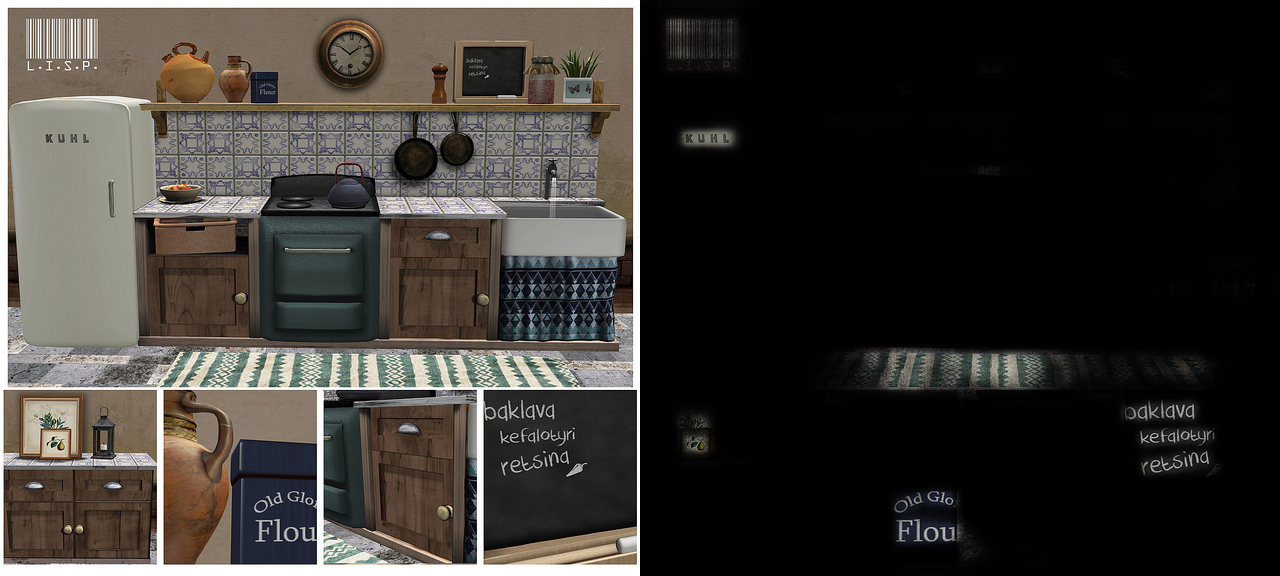
\includegraphics[width=\textwidth]{coco60kpred.png}
	\caption{Immagine originale e immagine combinata con mappa delle probabilità.}
\label{fig:coco_example}
\end{figure}

Osservando l'andamento della loss per tutte e le iterazioni si può notare un trend che farebbe pensare ad un overfitting sui dati, infatti da 60mila iterazioni in poi (circa 64 epoche\footnote{nonostante parlare di epoche abbia poco senso in quanto, come già spiegato nella sezione~\ref{subsubsec:gendata}, il training set è mutevole}) la loss su un sottoinsieme fisso del validation set rimane pressoché invariata mentre quella del training è in lenta discesa.

\begin{figure}[H]
	\centering
	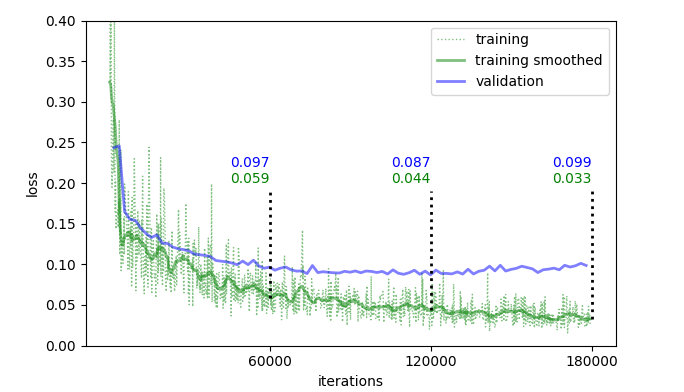
\includegraphics[width=\textwidth]{coco_loss.png}
	\caption{Curve di loss su training a validation set.}
\label{fig:coco_loss}
\end{figure}

Applicando invece l'algoritmo di estrazione delle bounding box con soglia 32 pixel ed infine valutando con \textit{Intersection over Union} a $0.5$, i miglioramenti vi sono, come si può notare dai risultati riportati nella tabella~\ref{tab:coco}.

\begin{table}[H]
\centering
\begin{threeparttable}
	\begin{tabular}{l*{5}c}
		\toprule
		\multirow{2}{*}{\textbf{Iterazioni}} & \multicolumn{3}{c}{\textbf{Recall}} & \multirow{2}{*}{\textbf{Precision}} & \multirow{2}{*}{\textbf{F1-score}} \\
		\cmidrule(lr){2-4}
		& Leggibili & Illegibili & Totale &  &  \\
		\midrule
		\multicolumn{6}{l}{Intero validation set} \\
		60k		& $16.21$ & $4.14$ & $12.28$ & $13.85$ & $13.01$ \\
		180k	& $20.87$ & $9.59$ & $17.29$ & $17.72$ & $17.50$ \\
		\midrule
		\multicolumn{6}{l}{Almeno un leggibile per immagine} \\
		60k		&   ---   & $3.41$ & $12.79$ & $24.11$ & $16.71$ \\
		180k	&   ---   & $9.00$ & $17.78$ & $28.15$ & $21.79$ \\
		\bottomrule
	\end{tabular}
	\begin{tablenotes}
		\item \footnotesize{Valori espressi in percentuale.}
	\end{tablenotes}
\end{threeparttable}
\caption{}\label{tab:coco}
\end{table}

%Non è ben chiaro dunque l'appiattimento della curva di loss su un sottoinsieme del validation set.


\subsection{Incidental Scene Text}
\label{subsec:train_inc}
I risultati già dopo le prime 60mila iterazioni (960 epoche) non sono promettenti, infatti si presentata un calo drastico nella precision rispetto a COCO-Text. Si confrontino i risultati riportati nella tabella~\ref{tab:incidental} con quelli della precedente tabella~\ref{tab:coco}.

\begin{table}[H]
\centering
\begin{threeparttable}
	\begin{tabular}{l*{5}c}
		\toprule
		\multirow{2}{*}{\textbf{Iterazioni}} & \multicolumn{3}{c}{\textbf{Recall}} & \multirow{2}{*}{\textbf{Precision}} & \multirow{2}{*}{\textbf{F1-score}} \\
		\cmidrule(lr){2-4}
		& Leggibili & Illegibili & Totale &  &  \\
		\midrule
		\multicolumn{6}{l}{Intero validation set} \\
		60k		& $19.07$ & $5.78$ & $14.54$ & $7.87$ & $10.21$ \\
		\midrule
		\multicolumn{6}{l}{Almeno un leggibile per immagine} \\
		60k		&   ---   & $5.69$ & $15.48$ & $13.95$ & $14.67$ \\
		\bottomrule
	\end{tabular}
	\begin{tablenotes}
		\item \footnotesize{Valori espressi in percentuale.}
	\end{tablenotes}
\end{threeparttable}
\caption{}\label{tab:incidental}
\end{table}


Il problema potrebbe essere imputabile alla groundtruth lievemente differente rispetto a quella di COCO-Text la quale presenta poche bounding box ruotate. Più avanti ritorneremo ad analizzare questo fenomeno.


\subsection{SynthText}
L'addestramento su questo dataset viene presto abbandonato ancora in fase sperimentale in quanto i risultati visivi (si veda la figura~\ref{fig:synth_example}) mostrano chiaramente un apprendimento poco significativo.\par

\begin{figure}[H]
	\centering
	\begin{subfigure}[b]{0.49\textwidth}
		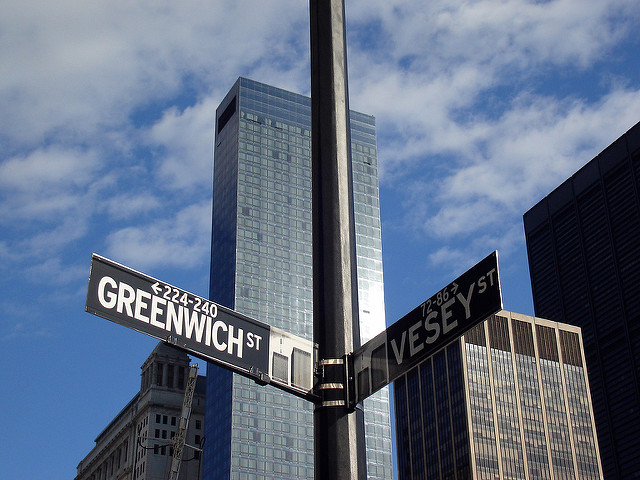
\includegraphics[width=\textwidth]{synth_original.png}
	\end{subfigure}
	\hfill
	\begin{subfigure}[b]{0.49\textwidth}
		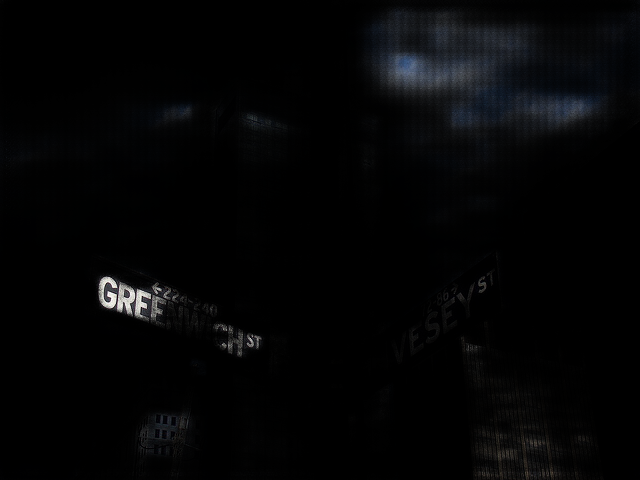
\includegraphics[width=\textwidth]{synth_mask.png}
	\end{subfigure}
\caption{}
\label{fig:synth_example}
\end{figure}

Il problema è molto probabilmente dovuto alla natura sintetica del dataset per cui molti elementi testuali, seppur posizionati tenendo conto della forma e perspettiva, si ritrovano in contesti completamente irreali e risultano dunque fuorvianti ai fini dell'addestramento della rete neurale.



\section{Modifiche strutturali}

I risultati ottenuti, seppur mostrino come questo approccio sia corretto nella forma, non raggiungono numeri soddisfacenti, l'obiettivo è dunque quello di cercare di migliorare senza però complicare il processo di estrazione delle bounding box illustrato nello pseudocodice~\ref{alg:bbox}. Ciò è dato dal fatto che il fine postoci è quello di adoperare principalmente una FCN, senza dunque ricorrere a metodi raffinati da porre in coda alla catena di elaborazione dei dati come effettuato da diversi altri metodi citati in precedenza nella sezione~\ref{sec:sota}.\par
Osservando le predizioni ottenute con l'addestramento su COCO-Text, si può notare come le zone di testo predette non siano molto raffinate e finiscano dunque per raggruppare insieme molte parole vicine fra di loro. Per ovviare a questo problema le soluzioni adottate che andremo a descrivere sono principalmente due:
\begin{itemize}
	\item
		Nuova classe ``bounding box'' che rappresenti il contorno di una parola.
	\item
		Nuova classe ``separazione'' che rappresenti una linea immaginaria che separi due parole vicine fra di loro.
\end{itemize}

In quanto difficilmente una \textit{Fully Convolutional Network} è in grado di generare una segmentazione raffinata in presenza di più classi, soprattutto quando queste sono simili o complementari, la generazione delle predizioni di aree testuali verrà effettuata come descritto nell'algoritmo~\ref{alg:sub_prob}, piuttosto che nel modo tradizionale con il quale si sceglierebbe la classe con score maggiore.

\begin{algorithm}
\caption{}\label{alg:sub_prob}
\begin{algorithmic}
	\State{$\textit{output} \gets \emptyset \in \mathbb{R}^{n \times m}$}
	\Comment{$\textit{probText, probThird} \in \mathbb{R}^{n \times m}$}
	\For{$i \textbf{ from } 1 \textbf{ to } n$}
		\For{$j \textbf{ from } 1 \textbf{ to } m$}
			\State{$\textit{value} \gets \textit{probText}[i][j] - \textit{probThird}[i][j]$}
			\If{$\textit{value} \geq \textit{threshold}$}
				\State{$\textit{output}[i][j] \gets \textit{value}$}
			\EndIf{}
		\EndFor{}
	\EndFor{}
	\Return{$\textit{output}$}
\end{algorithmic}
\end{algorithm}

dove \textit{probText} e \textit{probThird} sono rispettivamente mappe di probabilità di appartenenza alle classi di testo e bounding box / separazione, entrambe generate dopo l'applicazione della funzione di Softmax agli score finali.


\subsection{BranchFCN}
\label{subsec:train_branch}
Questa approccio deve il suo nome alla modifica apportata all'FCN fin'ora usata per contrastare un problema sorto in fase di implementazione. Infatti durante un addestramento preliminare si è notato che con l'introduzione della nuova classe delle bounding box le zone con probabilità di essere testo venivano ristrette producendo come effetto indesiderato l'annichilamento di tali predizioni ove il testo fosse di piccole dimensioni.\par
La soluzione consiste nello sdoppiare la fase di deconvoluzione finale in due rami, uno che generi predizioni per la solo area di testo ed il secondo per le sole bounding box. La scelta di ramificare dopo la fase di classificazione è dettata prettamente dal volere mantenere una certa efficenza, si evita infatti di raddoppiare il numero di pesi totali della rete (presenti perlopiù nella fase finale della VGG) e di addestrare due reti similari separate.\par
In aggiunta a ciò, l'operazione di \texttt{closing} utilizzata nell'algoritmo~\ref{alg:bbox} viene sostituita con un'operazione di \texttt{dilation} al fine di recuperare parte dei contorni persi durante l'applicazione dell'algoritmo~\ref{alg:sub_prob} precedentemente descritto.\par 
Come per il primo training su COCO-Text, anche con questo approccio si è deciso di addestrare la rete per 180mila iterazioni. I risultati visivi sono già da subito promettenti come mostrato nella figura~\ref{fig:branch_visualize}.

\begin{figure}[H]
	\centering
	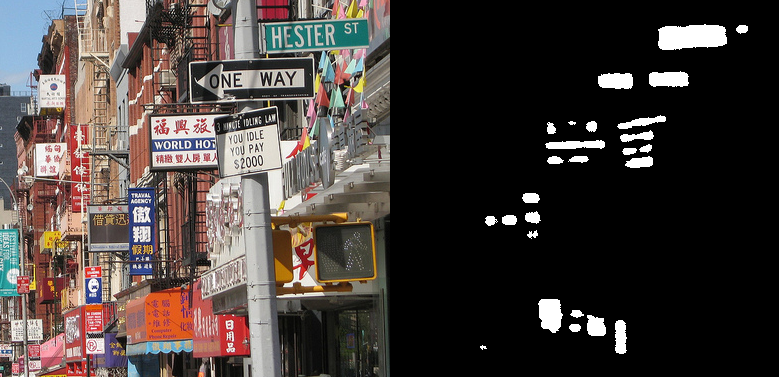
\includegraphics[width=0.9\textwidth]{branch_visualize.png}
	\caption{Immagine con relativa mappa delle probabilità.}
\label{fig:branch_visualize}
\end{figure}

Il grafico della funzione di loss (una media aritmetica fra i due rami dell'architettura) ci mostra come l'apprendimento non venga rallentato dalla presenza di una nuova classe in quanto i valori riflettono quanto già visto con l'addestramento di base su COCO-Text.

\begin{figure}[H]
	\centering
	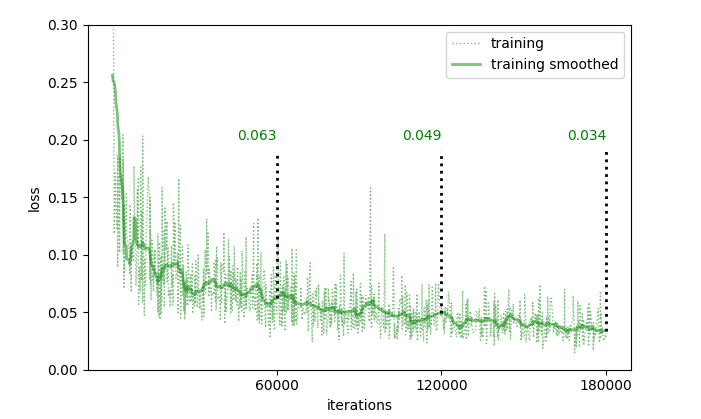
\includegraphics[width=\textwidth]{branch_loss.png}
	\caption{Curva di loss su training set.}
\label{fig:branch_loss}
\end{figure}

Nella tabella seguente~\ref{tab:branch} i risultati sul validation set, nella quale si può notare come i miglioramenti generali rispetto all'addestramento base siano notevoli seppur vi sia un lieve decremento nella recall su zone illeggibili.


\begin{table}[H]
\centering
\begin{threeparttable}
	\begin{tabular}{l*{5}c}
		\toprule
		\multirow{2}{*}{\textbf{Iterazioni}} & \multicolumn{3}{c}{\textbf{Recall}} & \multirow{2}{*}{\textbf{Precision}} & \multirow{2}{*}{\textbf{F1-score}} \\
		\cmidrule(lr){2-4}
		& Leggibili & Illegibili & Totale &  &  \\
		\midrule
		\multicolumn{6}{l}{Intero validation set} \\
		180k		& $35.91$ & $6.98$ & $26.13$ & $21.55$ & $23.62$ \\
		\midrule
		\multicolumn{6}{l}{Almeno un leggibile per immagine} \\
		180k		&   ---   & $6.74$ & $27.99$ & $35.46$ & $31.29$ \\
		\bottomrule
	\end{tabular}
	\begin{tablenotes}
		\item \footnotesize{Valori espressi in percentuale.}
	\end{tablenotes}
\end{threeparttable}
\caption{}\label{tab:branch}
\end{table}


\subsection{Word Division}
\label{subsec:train_wd}
Come approccio alternativo rimane quello di introduzione di una classe che rappresenti una linea immaginaria di separazione fra due parole abbastanza vicine. A differenza di BranchFCN però qui non è necessario modificare la rete neurale poiché, per come definita, la nuova classe non dovrebbe avere effetti collaterali sulle predizioni delle aree di testo.\par
V'è però il problema della definizione di un algoritmo per il posizionamento di questa nuova classe nell'immagine di groundtruth. La seguente figura~\ref{fig:division_proto} dovrebbe chiarire l'idea alla base dello pseudocodice~\ref{alg:drawsep}, il cui scopo è quello di rilevare i punti di intersezione esterni di due bounding box, compiendo delle espansioni qualora non fossero in contatto diretto.

\begin{figure}[H]
	\centering
	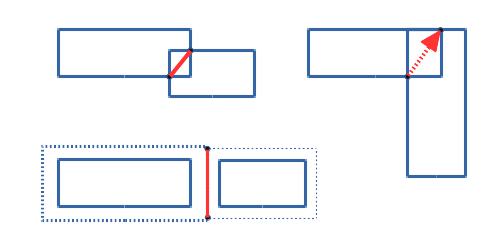
\includegraphics[width=0.8\textwidth]{division_proto.png}
	\caption{I tre esempi principali di estrazione della linea di separazione.}
\label{fig:division_proto}
\end{figure}

Nella seguente tabella~\ref{tab:word} i risultati sul validation set, non dissimili a quelli osservati in precedenza con BranchFCN.\par

\begin{table}[H]
\centering
\begin{threeparttable}
	\begin{tabular}{l*{5}c}
		\toprule
		\multirow{2}{*}{\textbf{Iterazioni}} & \multicolumn{3}{c}{\textbf{Recall}} & \multirow{2}{*}{\textbf{Precision}} & \multirow{2}{*}{\textbf{F1-score}} \\
		\cmidrule(lr){2-4}
		& Leggibili & Illegibili & Totale &  &  \\
		\midrule
		\multicolumn{6}{l}{Intero validation set} \\
		180k		& $38.88$ & $8.37$ & $28.70$ & $23.64$ & $25.94$ \\
		\midrule
		\multicolumn{6}{l}{Almeno un leggibile per immagine} \\
		180k		&   ---   & $7.84$ & $30.60$ & $36.74$ & $33.39$ \\
		\bottomrule
	\end{tabular}
	\begin{tablenotes}
		\item \footnotesize{Valori espressi in percentuale.}
	\end{tablenotes}
\end{threeparttable}
\caption{}\label{tab:word}
\end{table}


\begin{algorithm}[H]
\begin{algorithmic}
\caption{Calcolo e disegno linee di separazione.}\label{alg:drawsep}
\Function{DrawSeparations}{$\textit{gtImage, bboxes, nExpansion, thickness}$}
	\State{$\textit{intersected} \gets \emptyset$}
	\For{$i \textbf{ from } 0 \textbf{ to } \textit{nExpansion}$}
		\For{$b_1 \in \textit{bboxes}$}
			\For{$b_2 \in \textit{bboxes}$}
				\If{$(b_1, b_2) \notin \textit{intersected}$}
					\State{$\textit{line} \gets \Call{GetLine}{b_1 \textit{, } b_2}$}
					\If{$\textit{line} \neq \varnothing$}
						\State{$\textit{intersected} \gets \textit{intersected } \cup \{(b_1, b_2)\}$}
						\State{$\Call{DrawLine}{\textit{gtImage, line, thickness}}$}
					\EndIf{}
				\EndIf{}
			\EndFor{}
		\EndFor{}
		\For{$b \in \textit{bboxes}$}:
			\State{$b \gets \Call{expand}{b}$}
		\EndFor{}
	\EndFor{}
	\Return{$\textit{gtImage}$}
\EndFunction{}
\\
\Function{GetLine}{$b_1 \textit{, } b_2$}
	\If{$(b_1 \cap b_2 \neq \emptyset) \land (b_1 \nsubseteq b_2) \land (b_2 \nsubseteq b_1)$}
		\State{$\textit{inter} \gets b_1 \cap b_2$}
		\State{$\textit{union} \gets b_1 \cup b_2$}
		\If{$\textit{inter} \textbf{ is a Line}$}
			\Return{$\textit{inter}$}
		\Else{}
			\LineComment{Vertici su angoli concavi.}
			\State{$p \gets [v \mid \forall v \in \textit{union.verteces} : \Call{angle}{v} > 180^\circ]$}
			\If{$\Vert p \Vert = 1$}
				\LineComment{Annotationi unite a L $\Rightarrow$ vertice opposto al concavo}
				\Return{$p \cap \textit{inter.verteces}$}
			\ElsIf{$\Vert p \Vert = 0$}
				\LineComment{Annotazioni allineate $\Rightarrow$ best-fit line}
				\Return{$\Call{FitLine}{\textit{inter}}$}
			\ElsIf{$\Vert p \Vert = 4$}
				\LineComment{Annotazioni incrociate $\Rightarrow$ undefined}
				\Return{$\varnothing$}
			\Else{} \Comment{$\Vert p \Vert = 2$}
				\Return{$\Call{Line}{p[0] \textit{, } p[1]}$}
			\EndIf{}
		\EndIf{}
	\Else{}
		\Return{$\varnothing$}
	\EndIf{}
\EndFunction{}
\end{algorithmic}
\end{algorithm}


\begin{figure}[H]
	\centering
	\begin{subfigure}[b]{0.49\textwidth}
		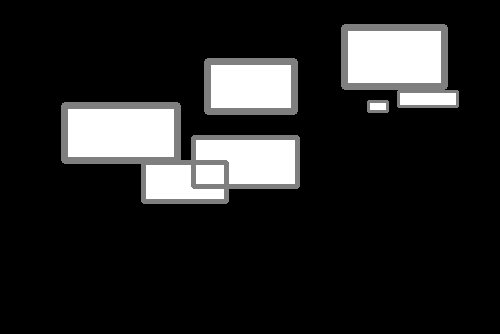
\includegraphics[width=\textwidth]{gt_branch.png}
		\caption{BranchFCN}
	\end{subfigure}
	\hfill
	\begin{subfigure}[b]{0.49\textwidth}
		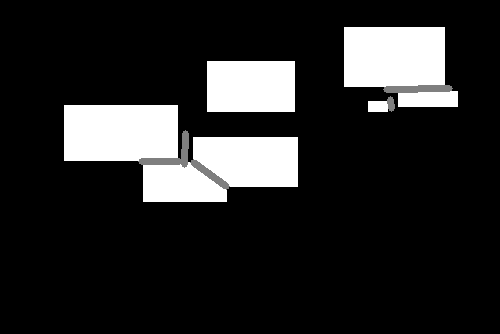
\includegraphics[width=\textwidth]{gt_word.png}
		\caption{Word Division}
	\end{subfigure}
	\caption{Immagini di groundtruth delle due varianti presentate.}
\end{figure}


\section{Finetuning e Data Augmentation}
Dopo aver cercato di migliorare l'accuratezza delle predizioni andando a modificare gli output della rete neurale e la rete stessa, per l'ottimizzazione del modello finale rimangono solo approcci quali il \textit{finetuning} e la \textit{data augmentation}, entrambi descritti nello specifico in seguito.


\subsection{Finetuning}
\label{subsec:train_fine}
Questa non è la prima volta in cui adottiamo questa tecnica, infatti come già accennato nella sezione~\ref{subsec:impl}, la parte iniziale dell'FCN da noi utilizzata fin'ora è stata sempre inizializzata con pesi derivanti da un precedente addestramento su un task generico di object classification.\par
Questo potrebbe destare dubbi sull'ottimalità dell'impostazione della rete, ma è stato ormai dimostrato come un approccio del genere sia del tutto sensato a fini di classificazione generale in più ambiti, portando a risparmiare risorse computazionali senza dover partire da un modello ex novo.\par
L'idea è dunque quella di continuare ad addestrare uno dei modelli da noi precedentemente descritti, nello specifico \textit{Word Division}, utilizzando nuovi dati provenienti da Incidental Scene Text.\par
Osservando l'andamento della curva di loss riportata nella figura~\ref{fig:finetune_loss}, i risultati appaiono ottimistici, tant'è che presto i valori vanno ad assestarsi fino a dimezzarsi dopo circa 40mila iterazioni.

\begin{figure}[H]
	\centering
	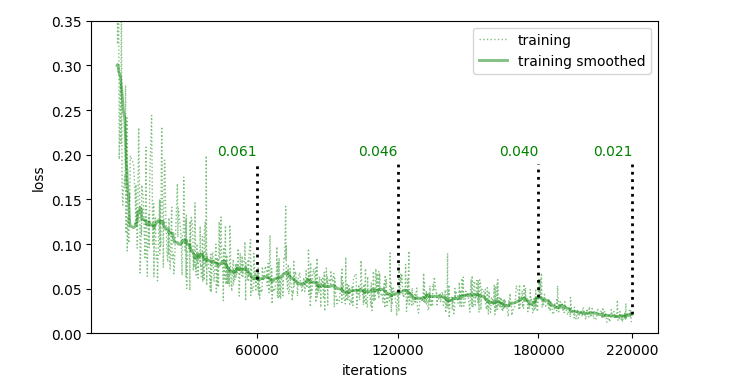
\includegraphics[width=0.95\textwidth]{finetune_loss.png}
	\caption{Curva di loss su COCO-Text prima e Incidental dopo.}
\label{fig:finetune_loss}
\end{figure}

\vfill
Purtroppo i risultati in validazione, riportati nella tabella~\ref{tab:finetune}, mostrano una realtà abbastanza diversa, anche se non a noi estranea.\par
Infatti, seppur la recall abbia un notevole incremento, lo stesso non si può dire della precision che, proprio come successo addestrando la rete da zero su Incidental Scene Text, tende a diminuire drasticamente. Ancora, questo comportamento non ha spiegazioni certe, l'unica ipotesi avanzata rimane quella della già citata differente natura delle annotazioni tra i due dataset.
\vfill

\begin{table}[H]
\centering
\begin{threeparttable}
	\begin{tabular}{l*{5}c}
		\toprule
		\multirow{2}{*}{\textbf{Iterazioni}} & \multicolumn{3}{c}{\textbf{Recall}} & \multirow{2}{*}{\textbf{Precision}} & \multirow{2}{*}{\textbf{F1-score}} \\
		\cmidrule(lr){2-4}
		& Leggibili & Illegibili & Totale &  &  \\
		\midrule
		\multicolumn{6}{l}{Intero validation set} \\
		180k		& $16.21$ & $4.14$  & $12.28$ & $13.85$ & $13.01$ \\
		220k		& $24.99$ & $11.26$ & $20.54$ & $11.95$ & $15.11$ \\
		\midrule
		\multicolumn{6}{l}{Almeno un leggibile per immagine} \\
		180k		&   ---   & $3.41$ & $12.79$ & $24.11$ & $16.71$ \\
		220k		&   ---   & $7.84$ & $21.55$ & $19.94$ & $20.72$ \\
		\bottomrule
	\end{tabular}
	\begin{tablenotes}
		\item \footnotesize{Valori espressi in percentuale.}
	\end{tablenotes}
\end{threeparttable}
\caption{}\label{tab:finetune}
\end{table}


\subsection{Data Augmentation}
\label{subsec:train_cocoaug}
Tale approccio consiste nell'aumentare la quantità di dati disponibile da fornire alla rete neurale manipolando quelli già in nostro possesso. Anche questa idea non dovrebbe giungere nuova, infatti già nell'algoritmo~\ref{alg:gendata} di generazione di ritagli randomici viene adottata una tecnica simile, in quanto per qualsiasi immagine non solo vi possono essere tanti ritagli quante le annotazioni, ma possono esservene di molteplici anche per la stessa parola.\par
Scopo di questo nuovo sviluppo è dunque quello di introdurre nuove forme di \textit{data augmentation}, illustrate nella figura~\ref{fig:data_aug}, nello specifico:
\begin{itemize}
	\item
		Scambio dei canali RGB
	\item
		Rotazione di un angolo tra $[-\theta, \theta]$
\end{itemize}

Come primo tentativo vengono applicate entrambe le trasformazioni sempre su COCO-Text, ponendo $\theta = 45\text{\textdegree}$, utilizzando una FCN base. Già i primi risultati a 60mila iterazioni riportati nella tabella~\ref{tab:cocoaug} evidenziano un comportamento già incontrato, ovvero il calo nella precisione rispetto al metodo di base.

\begin{table}[H]
\centering
\begin{threeparttable}
	\begin{tabular}{l*{5}c}
		\toprule
		\multirow{2}{*}{\textbf{Iterazioni}} & \multicolumn{3}{c}{\textbf{Recall}} & \multirow{2}{*}{\textbf{Precision}} & \multirow{2}{*}{\textbf{F1-score}} \\
		\cmidrule(lr){2-4}
		& Leggibili & Illegibili & Totale &  &  \\
		\midrule
		\multicolumn{6}{l}{Intero validation set} \\
		60k		& $15.39$ & $6.66$  & $12.53$ & $7.29$ & $9.22$ \\
		\midrule
		\multicolumn{6}{l}{Almeno un leggibile per immagine} \\
		60k		&   ---   & $5.70$ & $12.82$ & $14.53$ & $13.62$ \\
		\bottomrule
	\end{tabular}
	\begin{tablenotes}
		\item \footnotesize{Valori espressi in percentuale.}
	\end{tablenotes}
\end{threeparttable}
\caption{}\label{tab:cocoaug}
\end{table}

\begin{figure}[H]
	\centering
	\begin{subfigure}[b]{0.23\textwidth}
		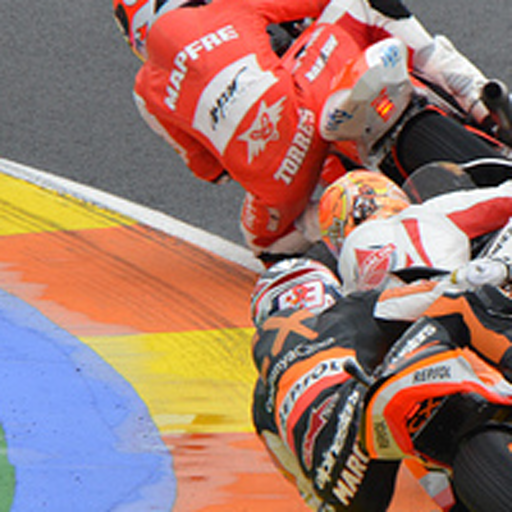
\includegraphics[width=\textwidth]{data_aug1.png}
		\caption{Originale}
	\end{subfigure}
	\hfill
	\begin{subfigure}[b]{0.23\textwidth}
		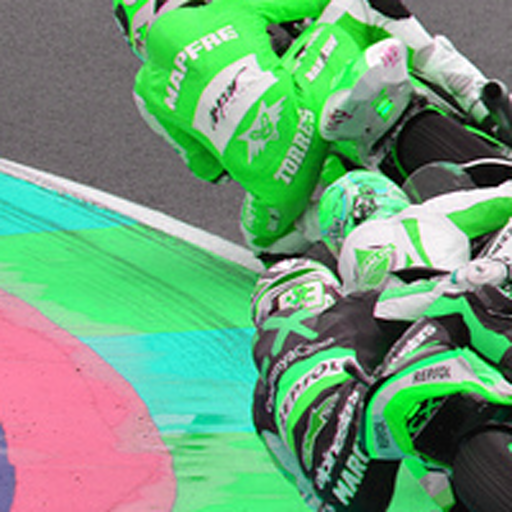
\includegraphics[width=\textwidth]{data_aug2.png}
		\caption{Scambio canali}
	\end{subfigure}
	\hfill
	\begin{subfigure}[b]{0.23\textwidth}
		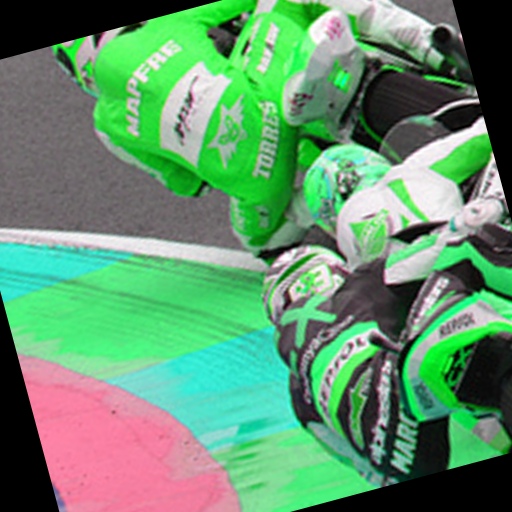
\includegraphics[width=\textwidth]{data_aug3.png}
		\caption{Rotazione}
	\end{subfigure}
\caption{}
\label{fig:data_aug}
\end{figure}


Questi risultati però ci permettono di indicare una possibile causa di questi fenomeni. Gli unici fattori imputabili sono infatti le trasformazioni applicate al dataset, e tra queste solo la rotazione potrebbe portare a somiglianze con Incidental Scene Text, il quale, a differenza di COCO-Text, presenta annotazioni precise sempre ruotate di qualche grado rispetto agli assi verticali e orizzontali.




\subsection{Confronto tra trasformazioni}
\label{subsec:train_wdaug}
Dati i risultati del precedente esperimento si è deciso di optare per questo nuovo tentativo di procedere con due approcci differenti da confrontare. 
\begin{itemize}
	\item
		Scambio canali RGB
	\item
		Scambio canali RGB + Rotazione $\theta = 15\text{\textdegree}$
\end{itemize}

La motivazione di questa scelta risiede nella volontà di testare quanto possa influire la rotazione, anche se minima, sulle performance finali. In aggiunta a ciò si passerà ad utilizzare come modello base \textit{Word Division} e l'addestramento partirà in finetuning su quest'ultimo da 120mila iterazioni fino a 180mila.\par
Confrontando i nuovi risultati nella tabella~\ref{tab:wdaug} con quelli ottenuti su \textit{Word Division} di base nella tabella~\ref{tab:word}, possiamo notare come le differenze prestazionali siano minime e come la precision tenda sempre a calare (anche se impercettibilmente con $\theta = 15\text{\textdegree}$) in favore di una migliore recall.

\begin{table}[H]
\centering
\begin{threeparttable}
	\begin{tabular}{l*{5}c}
		\toprule
		\multirow{2}{*}{\textbf{Iterazioni}} & \multicolumn{3}{c}{\textbf{Recall}} & \multirow{2}{*}{\textbf{Precision}} & \multirow{2}{*}{\textbf{F1-score}} \\
		\cmidrule(lr){2-4}
		& Leggibili & Illegibili & Totale &  &  \\
		\midrule
		\multicolumn{6}{l}{Intero validation set} \\
		Shuffle		& $38.34$ & $8.96$ & $28.52$ & $25.40$ & $26.87$ \\
		Shuffle+15	& $40.39$ & $7.78$ & $29.43$ & $24.70$ & $26.86$ \\
		\midrule
		\multicolumn{6}{l}{Almeno un leggibile per immagine} \\
		Shuffle		&   ---   & $8.40$ & $30.30$ & $37.06$ & $33.34$ \\
		Shuffle+15	&   ---   & $7.16$ & $31.34$ & $36.60$ & $33.80$ \\
		\bottomrule
	\end{tabular}
	\begin{tablenotes}
		\item \footnotesize{Valori espressi in percentuale.}
	\end{tablenotes}
\end{threeparttable}
\caption{}\label{tab:wdaug}
\end{table}


\subsection{Addestramento finale}
\label{subsec:train_final}
Infine, per l'ultimo addestramento si è deciso di utilizzare nuovamente \textit{Word Division} applicando sul dataset lo scambio dei canali RGB e la rotazione di $15\text{\textdegree}$, in quanto questo è l'approccio che fin'ora ha raggiunto risultati mediamente migliori. A differenza di quanto fatto in precedenza però il training ripartirà da zero sempre fino a 180mila iterazionni.\par
Nella tabella~\ref{tab:wdfinal} riportante i risultati finali è possibile notare come nella localizzazione di zone di aree di testo leggibili questo nuovo metodo si posizioni al di sopra di tutti gli altri, mentre complessivamente raggiunge la terza posizione, superato dai due metodi descritti nella sezione precedente~\ref{subsec:train_wdaug}. Le differenze nelle performance risultano comunque non significative. 


\begin{table}[H]
\centering
\begin{threeparttable}
	\begin{tabular}{l*{5}c}
		\toprule
		\multirow{2}{*}{\textbf{Iterazioni}} & \multicolumn{3}{c}{\textbf{Recall}} & \multirow{2}{*}{\textbf{Precision}} & \multirow{2}{*}{\textbf{F1-score}} \\
		\cmidrule(lr){2-4}
		& Leggibili & Illegibili & Totale &  &  \\
		\midrule
		\multicolumn{6}{l}{Intero validation set} \\
		180k		& $39.58$ & $9.57$ & $29.51$ & $23.66$ & $26.26$ \\
		\midrule
		\multicolumn{6}{l}{Almeno un leggibile per immagine} \\
		180k		&   ---   & $8.99$ & $31.34$ & $36.84$ & $33.87$ \\
		\bottomrule
	\end{tabular}
	\begin{tablenotes}
		\item \footnotesize{Valori espressi in percentuale.}
	\end{tablenotes}
\end{threeparttable}
\caption{}\label{tab:wdfinal}
\end{table}


In conclusione è possibile affermare come gli ultimi tentativi di \textit{data augmentation} abbiano portato miglioramenti negligibili in quanto le operazioni applicate sono poco significative rispetto a quanto già fatto nel modello base con l'utilizzo dei ritagli dettati dalle annotazioni. 


\subsection{Tabelle riassuntive}
Di seguito riportati i risultati dei vari metodi sviluppati mostrando:
\begin{itemize}
	\item
		recall, precision e F1-score totali (tabella~\ref{tab:total_results})
	\item
		recall, precision, e F1-score solo su annotazioni leggibili (tabella~\ref{tab:legible_results})
	\item
		recall specifica per le varie classi (tabella~\ref{tab:results_recall})
\end{itemize}

\vfill

\begin{table}[H]
\centering
\resizebox{\columnwidth}{!}{%
\begin{threeparttable}
	\begin{tabular}{l *{2}c *{2}c >{\bf}c }
		\toprule
		
		\textbf{Dataset} & \textbf{Metodo} & \textbf{Iters}	&
		\textbf{Recall} & \textbf{Precision} & \textbf{F1-score} \\

		\midrule

		Incidental Scene Text & FCN & 60k
			& 14.54 & 7.87 & 10.21 \\ 
		COCO Shuffled 45\textdegree{} & FCN & 60k
			& 12.53 & 7.29 & 9.22 \\ 
		COCO-Text & FCN & 60k
			& 12.28 & 13.85 & 13.01 \\ 
		COCO-Text & FCN & 180k
			& 17.29 & 17.72 & 17.50 \\ 
		COCO + Incidental & FCN & 220k
			& 20.54 & 11.95 & 15.11 \\ 
		COCO-Text & BranchFCN & 180k
			& 26.13 & 21.55 & 23.62 \\ 
		COCO-Text & WordDivision & 180k
			& 28.70 & 23.64 & 25.94 \\ 
		COCO Shuffled & WordDivision & 180k
			& 28.52 & 25.40 & 26.87 \\ 
		COCO Shuffled 15\textdegree{} & WordDivision & 180k
			& 29.43 & 24.70 & 26.86 \\ 
		COCO Shuffled 15\textdegree{} & WordDivision & 180k	
			& 29.51 & 23.66 & 26.26 \\

		\bottomrule
	\end{tabular}
	\begin{tablenotes}
		\item \footnotesize{Valori espressi in percentuale.}
	\end{tablenotes}
\end{threeparttable}%
}
\caption{Risultati sull'intero validation set.}\label{tab:total_results}
\end{table}

\vfill

\begin{table}[H]
\centering
\resizebox{\columnwidth}{!}{%
\begin{threeparttable}
	\begin{tabular}{l *{2}c *{2}c >{\bf}c }
		\toprule
		
		\textbf{Dataset} & \textbf{Metodo} & \textbf{Iters}	&
		\textbf{Recall} & \textbf{Precision} & \textbf{F1-score} \\

		\midrule

		Incidental Scene Text & FCN & 60k
			& 15.48 & 13.95 & 14.67 \\ 
		COCO Shuffled 45\textdegree{} & FCN & 60k
			& 12.82 & 14.53 & 13.62 \\ 
		COCO-Text & FCN & 60k
			& 12.79 & 24.11 & 16.71 \\ 
		COCO-Text & FCN & 180k
			& 17.78 & 28.15 & 21.79 \\ 
		COCO + Incidental & FCN & 220k
			& 21.55 & 19.94 & 20.72 \\ 
		COCO-Text & BranchFCN & 180k
			& 27.99 & 35.46 & 31.29 \\ 
		COCO-Text & WordDivision & 180k
			& 30.60 & 36.74 & 33.39 \\ 
		COCO Shuffled & WordDivision & 180k
			& 30.30 & 37.06 & 33.34 \\ 
		COCO Shuffled 15\textdegree{} & WordDivision & 180k
			& 31.40 & 36.60 & 33.80 \\ 
		COCO Shuffled 15\textdegree{} & WordDivision & 180k	
			& 31.34 & 36.84 & 33.87 \\

		\bottomrule
	\end{tabular}
	\begin{tablenotes}
		\item \footnotesize{Valori espressi in percentuale.}
	\end{tablenotes}
\end{threeparttable}%
}
\caption{Risultati sulle sole annotazioni leggibili.}\label{tab:legible_results}
\end{table}

\vfill

\begin{sidewaystable}
\begin{table}[H]
\centering
\resizebox{\columnwidth}{!}{%
\begin{threeparttable}
	\begin{tabular}{l *{5}c >{\it\/}c *{3}c >{\it\/}c >{\bf}c }
		\toprule
		
		\multirow{3}{*}{\textbf{Dataset}}		&
		\multirow{3}{*}{\textbf{Metodo}}		&
		\multirow{3}{*}{\textbf{Iters}}			&
		\multicolumn{9}{c}{\textbf{Recall}}		\\

		\cmidrule(lr){4-12}
		& & & \multicolumn{4}{c}{Leggibili} & \multicolumn{4}{c}{Illeggibili} & \multirow{2}{*}{} \\ 

		\cmidrule(lr){4-7} \cmidrule(lr){8-11} 

		& & & MP$^1$ & HW$^2$ & OT$^3$ & & MP$^1$ & HW$^2$ & OT$^3$ & & \\ 

		\midrule

		Incidental Scene Text & FCN & 60k
			& 19.40 & 15.51 & 12.78 & 19.07 & 6.13 & 7.10 & 4.14 & 5.78 & 14.54 \\
		COCO Shuffled 45\textdegree{} & FCN & 60k
			& 15.46 & 14.78 & 13.57 & 15.39 & 7.27 & 9.51 & 3.73 & 6.66 & 12.53 \\
		COCO-Text & FCN & 60k
			& 16.56 & 10.78 & 12.72 & 16.21 & 4.57 & 6.04 & 2.03 & 4.14 & 12.28 \\
		COCO-Text & FCN & 180k
			& 21.13 & 16.15 & 19.39 & 20.87 & 10.72 & 10.17 & 5.05 & 9.59 & 17.29 \\
		COCO + Incidental & FCN & 220k
			& 25.31 & 20.54 & 20.73 & 24.99 & 12.29 & 13.06 & 6.95 & 11.26 & 20.54 \\
		COCO-Text & BranchFCN & 180k
			& 36.36 & 30.66 & 27.61 & 35.91 & 7.94 & 7.48 & 3.19 & 6.98 & 26.13 \\
		COCO-Text & WordDivision & 180k
			& 39.61 & 31.10 & 24.17 & 38.88 & 9.37 & 10.34 & 4.15 & 8.37 & 28.70 \\
		COCO Shuffled & WordDivision & 180k
			& 39.00 & 30.88 & 25.42 & 38.34 & 9.72 & 13.10 & 5.01 & 8.96 & 28.52 \\
		COCO Shuffled 15\textdegree{} & WordDivision & 180k
			& 41.01 & 33.33 & 28.73 & 40.39 & 8.59 & 9.38 & 4.29 & 7.78 & 29.43 \\
		COCO Shuffled 15\textdegree{} & WordDivision & 180k	
			& 40.18 & 32.84 & 28.33 & 39.58 & 10.55 & 12.00 & 5.25 & 9.57 & 29.51 \\

		\bottomrule
	\end{tabular}
	\begin{tablenotes}
		\item \footnotesize{Valori espressi in percentuale.}
		\item \footnotesize{$^1$ Machine Printed}
		\item \footnotesize{$^2$ Handwritten}
		\item \footnotesize{$^3$ Others}
	\end{tablenotes}
\end{threeparttable}%
}
\caption{Valori di recall per le diverse classi.}\label{tab:results_recall}
\end{table}
\end{sidewaystable}


\section{Confronto con lo stato dell'arte}
In quest'ultima parte verranno mostrati i risultati ottenuti sui test set a disposizione al fine di mettere alla prova i modelli da noi addestrati contro metodi sviluppati da terzi negli ultimi anni.\par
Dalla nostra parte, i modelli presi in considerazione sono: 
\begin{itemize}
	\item
		BranchFCN (sezione~\ref{subsec:train_branch})
	\item
		Word Division con dataset aumentato (sezione~\ref{subsec:train_final})
	\item
		BranchFCN con soglia 0.65 e doppia \texttt{dilation}
	\item
		Word Division con dataset aumentato con soglia 0.6
\end{itemize}

Gli ultimi due modelli citati non sono stati prima analizzati in quanto sono variazioni nate nel corso di questi ultimi test al fine di massimizzare le prestazioni su Incidental Scene Text. In aggiunta a ciò, gli input della rete sono ridimensionati a risoluzioni vicine a \texttt{640 $\times$ 480}, media delle immagini di COCO-Text, in quanto alte risoluzioni portano ad una perdita di accuratezza facendo risaltare dettagli fuorvianti.\par
Come già accennato i test set sono quelli di \textit{Incidental Scene Text} e \textit{Focused Scene Text}, mentre i metodi di terzi riportati saranno quelli dei vincitori delle rispettive edizioni di ICDAR (2015 e 2013 rispettivamente) più i vari contendenti che hanno ottenuti i migliori risultati durante le successive edizioni, seppur non ufficialmente.

\subsection{Incidental Scene Text}

\begin{table}[H]
\centering
\begin{threeparttable}
	\begin{tabular}{l *{2}c >{\bf}c }
		\toprule
		
		\textbf{Metodo} & \textbf{Recall} & \textbf{Precision} & \textbf{F1-score} \\

		\midrule

		BranchFCN
		& 33.75 & 44.34 & 38.33 \\
		BranchFCN Tweaked
		& 37.02 & 54.19 & 43.99 \\
		WordDivision
		& 34.52 & 38.65 & 36.47 \\
		WordDivision Tweaked
		& 35.29 & 42.62 & 38.61 \\
		\midrule

		\multicolumn{1}{r}{Top-4 2015~\cite{ICDAR2015results}} \\
		Stradvision-2
		& 36.74 & 77.46 & 49.84 \\
		StradVision-1
		& 46.27 & 53.39 & 49.57 \\
		NJU Text (Version2)	
		& 36.25 & 70.44 & 47.87 \\
		AJOU~\cite{ajou}
		& 46.94 & 47.26 & 47.10 \\
		\midrule

		\multicolumn{1}{r}{Top-3 2017~\cite{ICDAR2015results}} \\
		Baidu VIS
		& 83.39 & 93.62 & 88.21 \\
		SenseTime V3 
		& 84.83 & 90.82 & 87.73 \\
		Dahua-OCR V3
		& 83.44 & 91.31 & 87.19 \\

		\bottomrule
	\end{tabular}
	\begin{tablenotes}
		\item \footnotesize{Valori espressi in percentuale.}
	\end{tablenotes}
\end{threeparttable}
\caption{Risultati sull'intero validation set.}\label{tab:incidental_results}
\end{table}

Dai risultati riporati nella tabella~\ref{tab:incidental_results} è possibile notare come nel giro di pochi anni lo stato dell'arte sia avanzato in maniera considerevele, ma è doveroso sottolineare come i nostri risultati ottenuti con strumenti disponibili al pubblico già nel 2015, ci possano posizionare nella classifica di quell'anno in quinta posizione con \textit{BranchFCN Tweaked}, oppure in settima con il modello con parametri di base.\par
Da notare è l'inversione di performance tra \textit{BranchFCN} e \textit{Word Division} rispetto ai risultati ottenuti su COCO-Text in fase di validazione, soprattutto nelle loro versioni migliorate.

\subsection{Focused Scene Text}

\begin{table}[H]
\centering
\begin{threeparttable}
	\begin{tabular}{l *{2}c >{\bf}c }
		\toprule
		
		\textbf{Metodo} & \textbf{Recall} & \textbf{Precision} & \textbf{F1-score} \\

		\midrule

		BranchFCN
		& 66.03 & 59.95 & 62.84 \\	
		BranchFCN Tweaked
		& 74.52 & 66.61 & 70.34 \\
		WordDivision
		& 67.21 & 57.54 & 62.01 \\
		WordDivision Tweaked
		& 70.96 & 59.40 & 64.67 \\
		\midrule

		\multicolumn{1}{r}{Top-3 2013~\cite{ICDAR2013results}} \\
		2R\_NUS\_FAR
		& 68.95 & 74.46 & 71.60 \\
		USTB\_TexStar
		& 61.46 & 84.76 & 71.25 \\
		CASIA\_NLPR
		& 66.12 & 74.64 & 70.12 \\
		\midrule

		\multicolumn{1}{r}{Top-3 2015~\cite{ICDAR2013results}} \\
		VGGMaxNet\_cmb~\cite{vggmaxnet}
		& 78.08 & 90.09 & 83.66 \\
		VGGMaxNet\_025~\cite{vggmaxnet}
		& 79.82 & 87.58 & 83.52 \\
		VGGMaxNet\_013~\cite{vggmaxnet}
		& 76.53 & 90.50 & 82.93 \\
		\midrule

		\multicolumn{1}{r}{Top-3 2017~\cite{ICDAR2013results}} \\	
		SenseTime
		& 91.87 & 95.45 & 93.62 \\
		DLVCtext
		& 88.49 & 93.35 & 90.86 \\
		MultDet
		& 89.68 & 91.09 & 90.38 \\

		\bottomrule
	\end{tabular}
	\begin{tablenotes}
		\item \footnotesize{Valori espressi in percentuale.}
	\end{tablenotes}
\end{threeparttable}
\caption{Risultati sull'intero validation set.}\label{tab:focused_results}
\end{table}

Similmente a quanto osservato su Incidental Scene Text, nel tempo lo stato dell'arte è notevolmente avanzato e \textit{BranchFCN} è ancora in netto vantaggio rispetto a \textit{Word Division}, anche se solo nella sua versione modificata.\par
Questa volta però i nostri approcci non raggiungono risultati soddisfacenti, posizionandosi poco dietro i primi classificati nel 2013, ma ben lontani dai modelli concorrenti sviluppati fino al 2015.


\chapter{Conclusione e sviluppi futuri}

Questa tesi ha affrontato il problema della localizzazione del testo in immagini digitali con tecniche di \textit{deep learning}.\par
Come primo passo abbiamo presentato i dataset a nostra disposizione e i metodi di valutazione al fine di analizzare su quanto avremmo dovuto operare e quali obiettivi raggiungere. In seguito abbiamo descritto brevemente le reti neurali e la loro storia col fine di presentare lo strumento principale adottato in questa tesi per l'implementazone, descritta nell'ultima parte, di un nostro metodo per la \textbf{text localization}.\par


\section{Risultati}
L'architettura delle Fully Convolutional Networks è stata cruciale per lo sviluppo del nostro metodo e ci ha permesso di ottenere i risultati aspettati nonostante i dati di partenza scarsi o poco precisi, ma soprattutto differenti da quelli per cui è stata ideata inizialmente.\par 
Questa ha anche mostrato le sue limitazioni sulla precisione della granularità della segmentazione che ci ha obbligato a sviluppare approcci alternativi per superare la difficoltà nel separare parole distinte.\par
Nonostante questi limiti, il modello architetturale ci ha permesso di compiere con relativa semplicità la fase di localizzazione del testo classificandosi alla pari con metodi concorrenti più sofisticati sviluppati nel periodo in qui questa rete neurale è stata introdotta.


\section{Sviluppi futuri}
I risultati ottenuti però al contempo deludono rispetto ai numeri attualmente raggiunti dallo stato dell'arte. Ciò è da imputare principalmente al fatto che gli strumenti da noi utilizzati, seppur recenti, risultano ormai superati da nuovi sviluppi nella ricerca che continua a fare grandi passi.\par 
Andando a toccare su più frangenti i metodi da noi illustrati, di seguito sono descritti i vari miglioramenti che possono essere adottati, in ordine di complessità.

\subsubsection{Modifica Groundtruth}
Questo è un obiettivo che in parte abbiamo già sviluppato coi nostri tentativi di utilizzare una nuova classe da predire, ma le idee potrebbero essere molteplici. Fra queste possiamo citare un approccio visto nella già citata \textbf{WordFence}~\cite{polzounov2017wordfence}, ovvero utilizzare una maschera dei pesi per la loss pixel per pixel che faccia pesare di meno eventuali predizioni negative agli estremi delle bounding box. 

\subsubsection{Deconvoluzione}
Come già osservato nella sezione~\ref{sec:FCN} la fase di deconvoluzione è divisa in due passi per ritornare alla dimensione originale dell'input, in cui vengono addizionati due dei layer precedenti di pooling. L'idea sarebbe dunque quella di estendere questo procedimento tante volte quante le fasi di pooling in maniera da costruire una fase di deconvoluzione ``specchiata'' rispetto a quella di convoluzione.\par

\subsubsection{Classificatore}
Nella sezione~\ref{subsec:case_studies} abbiamo descritto in breve alcuni degli ultimi risultati nella modellazione di reti neurali convoluzionali, fra cui ricade anche la VGG utilizzata alla base delle Fully Convolutional Networks. Come è possibile notare, seppure questa sia il classificatore di riferimento, nulla impedirebbe di rimpiazzarla con uno dei modelli a lei superiori nel task di object detection, portando di conseguenza teoricamente a risultati più precisi. 

\subsubsection{Estrazione Bounding Box}
Infine come tentativo ultimo, anche se non meno importante, rimane quello di sviluppare un nuovo metodo più sofisticato rispetto a quello da noi utilizzato (che ricordiamo essere semplici operazioni morfologiche e di rilevamento di componenti connesse) da mettere in coda alla fase di segmentazione.\par
L'idea potrebbe essere quella di di utilizzare sempre un approccio orientato al machine learning ma questa volta di natura differente, per esempio un task di regressione delle bounding box come già accennato in precedenza nello stato dell'arte~\cite{he2017deep}.



\bibliographystyle{unsrt}
\bibliography{bibtex}

\end{document}
